\documentclass[11pt]{book}

\tolerance=600

% for \begin{center}, etc.
\usepackage[margin=1.0in]{geometry}

\usepackage{seqsplit}

% all kinds of math macros
\usepackage{amsmath}
\usepackage{amssymb}

% eps figures
\usepackage{epsfig}

% chapter title styles
\usepackage[Sonny]{fncychap}
\ChNameVar{\LARGE}
\ChTitleVar{\LARGE\sl}

% index
\usepackage{makeidx}
\makeindex


% part page style see
% http://tex.stackexchange.com/questions/6609/problems-with-part-labels-using-titlesec
\usepackage{titlesec}

\titleformat{\part}[display]
   {\Huge\filcenter}
   {{\partname{}} \thepart}
   {0em}
   {\hrule}



% hyperlinks -- load after fncychap
\usepackage{hyperref}

% color package
\usepackage[usenames]{color}

% longtable package used to split tables across pages
\usepackage{longtable}

% PDF-aware landscape package, used for rotating tables (including the
% longtable)
\usepackage{pdflscape}

% table coloring
\usepackage{colortbl}
\definecolor{tableShade}{rgb}{0.945,0.961,0.980}

% caption
\usepackage{caption}
\captionsetup[figure]{font=small,labelfont=small}

% make the MarginPars look pretty
\setlength{\marginparwidth}{0.75in}
\newcommand{\MarginPar}[1]{\marginpar{\vskip-\baselineskip\raggedright\tiny\sffamily
\hrule\smallskip{\color{red}#1}\par\smallskip\hrule}}

% to increase the likelihood that floats will occur "here" when you
% want them to
\renewcommand{\floatpagefraction}{1.0}
\renewcommand{\topfraction}{1.0}
\renewcommand{\bottomfraction}{1.0}
\renewcommand{\textfraction}{0.0}

% number subsubsections and put them in the TOC
\setcounter{tocdepth}{3}
\setcounter{secnumdepth}{3}

% custom hrule for title page
\newcommand{\HRule}{\rule{\linewidth}{0.125mm}}

% control sequences in verbatim
\usepackage{fancyvrb}

% short table of contents
\usepackage{shorttoc}

% spacing in the table of contents
\usepackage[titles]{tocloft}

\setlength{\cftbeforechapskip}{2ex}
\setlength{\cftbeforesecskip}{0.25ex}

% For splitting up lists into multitple columns
\usepackage{multicol}

% don't put a header on blank pages, see
% http://www.latex-community.org/forum/viewtopic.php?f=4&p=51559
% change ``plain'' to ``empty'' to eliminate the page number
\makeatletter
\renewcommand*\cleardoublepage{\clearpage\if@twoside
\ifodd\c@page\else
\hbox{}
\thispagestyle{empty}
\newpage
\if@twocolumn\hbox{}\newpage\fi\fi\fi}
\makeatother


% don't make the chapter/section headings uppercase.  See the fancyhdr
% documentation (section 9)
\usepackage{fancyhdr}
\renewcommand{\chaptermark}[1]{%
 \markboth{\chaptername
\ \thechapter.\ #1}{}}

\renewcommand{\sectionmark}[1]{\markright{\thesection---#1}}


% skip a bit of space between paragraphs, to enhance readability
\usepackage{parskip}



% special fraction
\newcommand{\sfrac}[2]{\mathchoice
  {\kern0em\raise.5ex\hbox{\the\scriptfont0 #1}\kern-.15em/
   \kern-.15em\lower.25ex\hbox{\the\scriptfont0 #2}}
  {\kern0em\raise.5ex\hbox{\the\scriptfont0 #1}\kern-.15em/
   \kern-.15em\lower.25ex\hbox{\the\scriptfont0 #2}}
  {\kern0em\raise.5ex\hbox{\the\scriptscriptfont0 #1}\kern-.2em/
   \kern-.15em\lower.25ex\hbox{\the\scriptscriptfont0 #2}}
  {#1\!/#2}}

\def\Ab {{\bf A}}
\def\eb {{\bf e}}
\def\Fb {{\bf F}}
\def\gb {{\bf g}}
\def\Hb {{\bf H}}
\def\ib {{\bf i}}
\def\Ib {{\bf I}}
\def\Kb {{\bf K}}
\def\lb {{\bf l}}
\def\Lb {{\bf L}}
\def\nb {{\bf n}}
\def\Pb {{\bf P}}
\def\Qb {{\bf Q}}
\def\rb {{\bf r}}
\def\Rb {{\bf R}}
\def\Sb {{\bf S}}
\def\ub {{\bf u}}
\def\Ub {{\bf U}}
\def\xb {{\bf x}}

\def\dt       {\Delta t}
\def\omegadot {\dot\omega}

\def\inp  {{\rm in}}
\def\outp {{\rm out}}
\def\sync {{\rm sync}}

\def\half   {\frac{1}{2}}
\def\myhalf {\sfrac{1}{2}}
\def\nph    {{n+\myhalf}}

% Level Set Macros
\def\ADDNODE       {{\tt{\bf ADDNODE}}}
\def\ADVANCE       {{\tt{\bf ADVANCE}}}
\def\done          {{\tt{\bf done}}}
\def\EVAL          {{\tt{\bf EVAL}}}
\def\INITPHI       {{\tt{\bf INITPHI}}}
\def\FASTMARCH     {{\tt{\bf FASTMARCH}}}
\def\FINDINTRFCE   {{\tt{\bf FINDINTRFCE}}}
\def\heap          {{\tt{\bf heap}}}
\def\heaploc       {{\tt{\bf heaploc}}}
\def\intface       {{\tt{\bf intface}}}
\def\intfacen      {{\tt{\bf intfacen}}}
\def\intfacenum    {{\tt{\bf intfacenum}}}
\def\intfacenumn   {{\tt{\bf intfacenumn}}}
\def\intfacenump   {{\tt{\bf intfacenump}}}
\def\intfacep      {{\tt{\bf intfacep}}}
\def\isnew         {{\tt{\bf isnew}}}
\def\LARGEINT      {{\tt{\bf LARGEINT}}}
\def\lvlerr        {{\tt{\bf lvlerr}}}
\def\LSCFL         {{\tt{\bf LSCFL}}}
\def\LStype        {{\tt{\bf LStype}}}
\def\LSnband       {{\tt{\bf LSnband}}}
\def\LSmine        {{\tt{\bf LSmine}}}
\def\mine          {{\tt{\bf mine}}}
\def\MINE          {{\tt{\bf MINE}}}
\def\mineloc       {{\tt{\bf mineloc}}}
\def\NARROWBAND    {{\tt{\bf NARROWBAND}}}
\def\nband         {{\tt{\bf nband}}}
\def\nbandnum      {{\tt{\bf nbandnum}}}
\def\nbandwidth    {{\tt{\bf nbandwidth}}}
\def\numtent       {{\tt{\bf numtent}}}
\def\PHIUPD        {{\tt{\bf PHIUPD}}}
\def\REINIT        {{\tt{\bf REINIT}}}
\def\RETYPIFY      {{\tt{\bf RETYPIFY}}}
\def\RMVNODE       {{\tt{\bf RMVNODE}}}
\def\sign          {{\tt{\bf sign}}}
\def\type          {{\tt{\bf type}}}
\def\UPDATE        {{\tt{\bf UPDATE}}}
\def\UPDATEF       {{\tt{\bf UPDATEF}}}
\def\UPDATENODE    {{\tt{\bf UPDATENODE}}}
\def\new           {{\rm new}}
\def\old           {{\rm old}}


\usepackage{listings}

\usepackage{subfig}

\definecolor{gray}{rgb}       {0.8,0.8,0.8}
\definecolor{light-blue}{rgb} {0.8,0.8,1.0}
\definecolor{light-green}{rgb}{0.8,1.0,0.8}
\definecolor{light-red}{rgb}  {1.0,0.9,0.9}

\lstset{frame=single,basicstyle=\footnotesize\ttfamily,showstringspaces=false,showspaces=false,xleftmargin=5pt,xrightmargin=6pt}

\lstset{language=C++,
                basicstyle=\footnotesize\ttfamily,
                keywordstyle=\color{blue}\footnotesize\ttfamily,
                commentstyle=\color{cyan}\footnotesize\ttfamily
}

\lstdefinelanguage{cpp}{
  language     = C++,
  morekeywords =
  [2]{amrex,amrex_real,
      Array,BaseFab,Box,BoxArray,DistributionMapping,FabArray,FArrayBox,
      Geometry,IArrayBox,IntVect,IndexType,MFIter,MultiFab,
      ParallelDescriptor,ParmParse,Real,RealBox,
      AMREX_SPACEDIM,AMREX_D_DECL},
  keywordstyle = [2]\color{red}\footnotesize\ttfamily,
}

% \lstset{
%   basicstyle=\small\ttfamily,%
%   frame=single,%
%   rulesepcolor=\color{gray},%
%   backgroundcolor=\color{white}%
% }
% \lstset{belowskip=-0.25em}


% Macros for indexing
\newcommand{\idxamrex}[1]{\index{\tt{amrex}!{\tt #1}}{\tt #1}}

%------------------------------------------------------------------------------
\input amrexsymbols
% \graphicspath{{Verification/}{Software/}{ConvertCheckpoint/}{Scaling/}{Visualization/}}


%------------------------------------------------------------------------------
\begin{document}



\frontmatter

\begin{titlepage}
\begin{center}
\ \\[3in]
{\sf \Huge AMReX}
\ \\[0.2in]

\begin{minipage}{5.5in}
\HRule\\[2mm]
\centering
{\Large \em An adaptive mesh refinement software framework}

\HRule
\end{minipage}

\ \\[.5 in]
{\sf \huge User's Guide}

\vfill

{\large AMReX Developers}
\ \\[0.3 in]
{\large \today}
\end{center}

\end{titlepage}


\shorttoc{Chapter Listing}{0}

\setcounter{tocdepth}{2}
\tableofcontents

\clearpage

\listoffigures
\addcontentsline{toc}{chapter}{list of figures}

\clearpage

\listoftables
\addcontentsline{toc}{chapter}{list of tables}


\cleardoublepage

\chapter*{Preface}
\addcontentsline{toc}{chapter}{Preface}
\input{Preface/Preface}

\mainmatter

\chapter{Introduction}\label{Chap:Introduction}
\amrex\ is a publicly available software framework designed for
building massively parallel block-structured adaptive mesh refinement
(AMR) applications.

Key features of \amrex\ include:
\begin{itemize}
\item \cpp\ and Fortran interfaces
\item 1-, 2- and 3-D support
\item Support for cell-centered, face-centered, edge-centered, and
  nodal data
\item Support for hyperbolic, parabolic, and elliptic solves on
  hierarchical adaptive grid structure
\item Optional subcycling in time for time-dependent PDEs
\item Support for particles
\item Parallelization via flat MPI, hybrid MPI/OpenMP, or MPI/MPI
\item Parallel I/O
\item Plotfile format supported by \amrvis, \visit, \paraview, and \yt.
\end{itemize}

Because \amrex's core is mainly written in \cpp, the basics of \amrex\
is first introduced in \cpp\ and then their Fortran wrappers if
available will be described as well.  

Besides the User's Guide, there is document generated by Doxygen at
\url{https://ccse.lbl.gov/pub/AMReX_Docs/}.  Documentation on
migration from \boxlib\ is available at {\tt Docs/Migration}.


\chapter{Getting Started}\label{Chap:GettingStarted}
In this chapter, we will walk you through two simple examples.  It is
assumed here that your machine has GNU Make, Python, GCC (including
gfortran), and MPI, although \amrex\ can be built with CMake and other
compilers. 

\section{Downloading the Code}

The source code of \amrex\ is available at
\url{https://github.com/AMReX-Codes/amrex}.  The GitHub repo is our
central repo for development.  The {\tt development} branch
includes the latest state of the code, and it is merged into the {\tt
  master} branch on a monthly basis.  The {\tt master} branch is
considered the release branch.  The releases are tagged with version
number {\tt YY.MM} (e.g., {\tt 17.04}).  The {\tt MM} part of the
version is incremented every month, and the {\tt YY} part every year.
Bug fix releases are tagged with {\tt YY.MM.patch} (e.g., {\tt
  17.04.1}).

\section{Example: Hello World}

The source code of this example is at {\tt
  amrex/Tutorials/Basic/HelloWorld\_C/} and is also shown below. 

\begin{lstlisting}[language=cpp]
 #include <AMReX.H>
 #include <AMReX_Print.H>

 int main(int argc, char* argv[])
 {
     amrex::Initialize(argc,argv);
     amrex::Print() << "Hello world from AMReX version " 
                    << amrex::Version() << "\n";
     amrex::Finalize();
 }
\end{lstlisting}

The main body of this short example contains three statements.
Usually the first and last statements for the {\tt main} function of
every program should be calling {\tt amrex::}\idxamrex{Initialize} and
\idxamrex{Finalize}, respectively.  The second statement calls {\tt
  amrex::}\idxamrex{Print} to print out a string that includes the
\amrex\ version returned by the {\tt amrex::}\idxamrex{Version}
function.  The example code includes two \amrex\ header files.  Note
that the name of all \amrex\ header files starts with {\tt AMReX\_}
(or just {\tt AMReX} in the case of {\tt AMReX.H}).  All \amrex\
\cpp\ functions are in the {\tt amrex} namespace.  

\subsection{Building the Code}

You build the code in the {\tt amrex/Tutorials/Basic/HelloWorld\_C/}
directory.  Typing {\tt make} will start the compilation process and
result in an executable named {\tt main3d.gnu.DEBUG.ex}.  The name
shows that the GNU compiler with debug options set by \amrex\ is used.
It also shows that the executable is built for 3D.  Although this
simple example code is dimension independent, the dimension matters
for all non-trivial examples.  The build process can be adjusted by
modifying the {\tt amrex/Tutorials/Basic/HellWorld\_C/GNUmakefile} file.
More details on how to build \amrex can be found in
Chapter~\ref{Chap:BuildingAMReX}.

\subsection{Running the Code}

The example code can be run as follows,
\begin{verbatim}
  ./main3d.gnu.DEBUG.ex
\end{verbatim}
The result may look like,
\begin{verbatim}
  Hello world from AMReX version 17.05-30-g5775aed933c4-dirty
\end{verbatim}
The version string means the current commit {\tt 5775aed933c4} (note
that there is no {\tt g}) is based on {\tt 17.05} with 30 additional
commits and the \amrex\ work tree is dirty (i.e. there are uncommitted
changes).

\subsection{Parallelization}

Now let's build with MPI by typing {\tt make USE\_MPI=TRUE}.  This
should make an executable named {\tt main3d.gnu.DEBUG.MPI.ex}.  Note
{\tt MPI} in the file name.  You can then run,
\begin{verbatim}
  mpiexec -n 4 ./main3d.gnu.DEBUG.MPI.ex
\end{verbatim}
The result may look like,
\begin{verbatim}
  MPI initialized with 4 MPI processes
  Hello world from AMReX version 17.05-30-g5775aed933c4-dirty
\end{verbatim}

If the compilation fails, you are referred to
Chapter~\ref{Chap:BuildingAMReX} on how to configure the build
system.

\section{Example: Heat Equation Solver}\label{sec:heat equation}

We now look at a more complicated example at {\tt
  amrex/Tutorials/Basic/HeatEquation\_EX1\_C} and show how simulation
results can be visualized.  Don't worry about the details of the code.
You will be able to understand the code in this example after
Chapter~\ref{Chap:Basics}. 

\subsection{Building and Running the Code}

To build a 2D executable, type {\tt make DIM=2}.  This will generate
an executable named {\tt main2d.gnu.ex}.  To run it, type,
\begin{verbatim}
  ./main2d.gnu.DEBUG.ex inputs_2d
\end{verbatim}
Note that the command takes a file {\tt inputs\_2d}.  When the run
finishes, you will have a number of plotfiles, {\tt plt00000}, {\tt
  plt01000}, etc.  The calculation solves the heat equation in 2D on a
$256 \times 256$ cells domain.  It runs $10,000$ steps and makes a
plotfile every $1,000$ steps.  These are runtime parameters that can
be adjusted in {\tt inputs\_2d}.

\section{Visualization}
There are several visualization tools that can be used for \amrex\
plotfiles.  The standard tool used within the
\amrex-community is \amrvis, a package developed and supported 
by CCSE that is designed specifically for highly efficient visualization
of block-structured hierarchical AMR data.
Plotfiles can also be viewed using the \visit, \paraview, and \yt packages.
Particle data can be viewed using \paraview.
Refer to Chapter \ref{Chap:Visualization} for how to use each of these tools.


\chapter{Building AMReX}\label{Chap:BuildingAMReX}

In this chapter, we discuss \amrex's build systems.  There are three
ways to use \amrex.  The approach used by \amrex\ developers uses GNU
Make.  There is no installation step in this approach.  Application
codes adopt \amrex's build system and compile \amrex\ while compiling
their own codes.  This will be discussed in more details in
Section~\ref{sec:build:make}.  The second approach is to build \amrex\
into a library and install it (Section~\ref{sec:build:lib}).  Then an
application code uses its own build system and links \amrex\ as an
external library.  \amrex\ can also be built with CMake
(Section~\ref{sec:build:cmake}).

\section{Building with GNU Make}
\label{sec:build:make}

In this build approach, you write your own make files defining a
number of variables and rules.  Then you invoke {\tt make} to start
the building process.  This will result in an executable upon
successful completion.  The temporary files generated in the building
process are stored in a temporary directory named {\tt
  tmp\_build\_dir}.

\subsection{Dissecting a Simple Make File}

An example of building with GNU Make can be found in {\tt
  amrex/Tutorials/Basic/HelloWorld\_C}.  Table~\ref{tab:makevarimp}
shows a list of important variables.
\begin{table}[t]
  \centering
  \begin{tabular}{lcc}
    Variable & Value & Default \\
    \hline
    {\tt AMREX\_HOME} & Path to amrex & environment \\
    {\tt COMP} & {\tt gnu}, {\tt cray}, {\tt intel}, {\tt llvm}, or {\tt pgi} & none \\
    {\tt DEBUG} & {\tt TRUE} or {\tt FALSE} & {\tt TRUE} \\
    {\tt DIM} & 1 or 2 or 3 & none \\
    {\tt USE\_MPI} & {\tt TRUE} or {\tt FALSE} & {\tt FALSE} \\
    {\tt USE\_OMP} & {\tt TRUE} or {\tt FALSE} & {\tt FALSE} \\
    \hline
  \end{tabular}
  \caption{\label{tab:makevarimp} Important make variables}
\end{table}

At the beginning of {\tt
  amrex/Tutorials/Basic/HelloWorld\_C/GNUmakefile}, {\tt AMREX\_HOME}
is set to the path to the top directory of \amrex.  Note that in the
example {\tt ?=} is a conditional variable assignment operator that
only has an effect if {\tt AMREX\_HOME} has not been defined
(including in the environment).  One can also set it through
environment variable.  For example in bash, one can set {\tt export
  AMREX\_HOME=/path/to/amrex}.

One must set the {\tt COMP} variable to choose a compiler.  Currently
the list of supported compilers includes {\tt gnu}, {\tt cray}, {\tt
  intel}, {\tt llvm}, and {\tt pgi}.  One must also set the {\tt DIM}
variable to either 1, 2, or 3, depending on the dimensionality of the
problem. 

Variables {\tt DEBUG}, {\tt USE\_MPI} and {\tt USE\_OMP} are optional
with default set to {\tt TRUE}, {\tt FALSE} and {\tt FALSE},
respectively.  The meaning of these variables should be obvious.  In
{\tt DEBUG} build, aggressive compiler optimization flags are turned
off and assertions in \amrex\ source code are turned on.  For
production runs, {\tt DEBUG} should be set to {\tt FALSE}.

After defining these make variables, a number of files, {\tt
  Make.defs}, {\tt Make.package} and {\tt Make.rules}, are included in
{\tt GNUmakefile}.  \amrex\ are split into a number of packages.  An
application code does not include every package.  In this simple
example, we only need to include {\tt
  \$(AMREX\_HOME)/Src/Base/Make.package}.  An application code also
has its own {\tt Make.package} file (e.g., {\tt ./Make.package} in
this example) to append source files to the build system using
operator {\tt +=}.  Variables for various source files are shown
below.
\begin{quote}
\begin{description}
\item [{CEXE\_sources}] \cpp\ source files.  Note that \cpp\
  source files are assumed to have a {\tt .cpp} extension.
\item [{CEXE\_headers}] \cpp\ headers with {\tt .h} or {\tt .H} extension.
\item [{cEXE\_sources}] C source files with {\tt .c} extension.
\item [{cEXE\_headers}] C headers with {\tt .h} extension.
\item [{f90EXE\_sources}] Free format Fortran source with {\tt
    .f90} extension.
\item [{F90EXE\_sources}] Free format Fortran source with {\tt
    .F90} extension.  Note that these Fortran files will go through
  preprocessing.
\end{description}
\end{quote}
In this simple example, the extra source file, {\tt main.cpp} is in
the current directory that is already in the build system's search
path.  If this example has files in a subdirectory (e.g., {\tt
  mysrcdir}), you will then need to add the following to {\tt
  Make.package}. 
\begin{verbatim}
    VPATH_LOCATIONS += mysrcdir
    INCLUDE_LOCATIONS += mysrcdir
\end{verbatim}
Here {\tt VPATH\_LOCATIONS} and {\tt INCLUDE\_LOCATIONS} are the search
path for source and header files, respectively.

\subsection{Tweaking Make System}

The GNU Make build system is located at {\tt amrex/Tools/GNUMake}.
You can read {\tt README.md} and the make files there for more
information.  Here we will give a brief overview.

Besides building executable, other common make commands include:
\begin{quote}
\begin{description}
  \item[make clean] This removes the executable, {\tt .o} files, and
    the temporarily generated files.  Note that one can add additional
    targets to this rule by using the double colon (::)
  \item[make realclean] This removes all files generated by make.
  \item[make help] This shows the rules for compilation.
  \item[make print-xxx] shows the value of varible {\tt xxx}.  This is
    very useful for debugging and tweaking the make system.
\end{description}
\end{quote}

Compiler flags are set in {\tt amrex/Tools/GNUMake/comps/}.  Note that
variables like {\tt CC} and {\tt CFLAGS} are reset in that directory
and their values in environment variables are disregarded. Site
specific setups (e.g., MPI installation) are in {\tt
  amrex/Tools/GNUMake/sites/}, which includes a generic setup in {\tt
  Make.unknown}.  You can override the setup by having your own {\tt
  Make.\$(host\_name)} file, where variable {\tt host\_name} is your
host name in the make system and can be found via {\tt make
  print-host\_name}.  You can also have a {\tt
  amrex/Tools/GNUMake/Make.local} file to override various variables.
See {\tt amrex/Tools/GNUMake/Make.local.template} for an example.

\section{Building {\tt libamrex}}
\label{sec:build:lib}

If an application code already has its own elaborated build system and
wants to use \amrex\ as an external library, this might be your
choice.  In this approach, one runs {\tt ./configure}, followed by
{\tt make} and {\tt make install}.  In the top \amrex\ directory, one
can run {\tt ./configure -h} to show the various options for the {\tt
  configure} script.  This approach is built on the \amrex\ GNU Make
system.  Thus Section~\ref{sec:build:make} is recommended if any fine
tuning is needed.

\section{Building with CMake}
\label{sec:build:cmake}

An alternative to the approach described in Section~\ref{sec:build:lib}
is to install \amrex\ as an external library by using the CMake build system.
A CMake build is a two-steps process. First {\tt cmake} is invoked to create 
configuration files and makefiles in a chosen directory ({\tt builddir}). 
This is roughly equivalent to running  {\tt ./configure} (see Section
~\ref{sec:build:lib}). Next, the actual build and installation are performed
by issuing {\tt make install} from within {\tt builddir}. This will install
the library files in a chosen installation directory ({\tt installdir}).
The CMake build process is summarized as follow:
\begin{verbatim}
export AMREX_HOME=/path/to/installdir
mkdir /path/to/builddir
cd    /path/to/builddir
cmake [options] -DCMAKE_INSTALL_PREFIX:PATH=$AMREX_HOME  /path/to/amrex 
make install
\end{verbatim} 
In the above snippet, {\tt [options]} indicates one or more options for the customization
of the build, as described in Subsection~\ref{sec:build:cmake:options}. It should be
 emphasized that {\tt AMREX\_HOME} is set to point to the desired installation 
directory, and {\bf NOT} to the \amrex\ source directory as for the GNU Make build.
 Although the \amrex\ source could be used as build directory, we advise against doing so.
After the installation is complete, {\tt builddir} can be removed.
\subsection{Customization options}
\label{sec:build:cmake:options}
\amrex\ configuration settings may be specified on the command line with the {\tt -D} option.
For example one can enable OpenMP support as follows:
\begin{verbatim}
cmake -DENABLE_OpenMP=1 -DCMAKE_INSTALL_PREFIX:PATH=$AMREX_HOME  /path/to/amrex 
\end{verbatim} 
The list of available option is reported in Table~\ref{tab:cmakevar}.
\begin{table}[h!]
  \centering
  \begin{tabular}{llcc}
    Option name & Description & Default Value & Possible values  \\
    \hline
    {\tt BL\_SPACEDIM} & Dimension of \amrex\ build & 3 & 2,3 \\
    {\tt ENABLE\_MPI} & Enable build with MPI & 1 & 0,1 \\
    {\tt ENABLE\_OpenMP} & Enable build with OpenMP & 0 & 0,1 \\
    {\tt BL\_USE\_PARTICLES} & Include particle classes in \amrex\ build & 0  & 0,1 \\
    {\tt ENABLE\_PROFILING} &  Include profiling info in \amrex\ build & 0  & 0,1 \\
    {\tt ENABLE\_BACKTRACE} & Include backtrace info in \amrex\ build & 1  & 0,1 \\
    \hline
  \end{tabular}
  \caption{\label{tab:cmakevar} Variables for the customization of \amrex\ build with CMake}
\end{table}





\chapter{{\tt Base} Source Code}\label{Chap:Basics}
In this chapter, we present the basics of \amrex.  The implementation
source codes are in {\tt amrex/Src/Base/}.  Note that \amrex\ classes
and functions are in namespace {\tt amrex}.  For clarity, we usually
drop {\tt amrex::} in the example codes here.  It is also assumed that
headers have been properly {\tt include}d.  We recommend you study
tutorials at {\tt amrex/Tutorials/Basic/} while reading this chapter.
After reading this chapter, one should be able to develop single-level
parallel codes using \amrex.  It should also be noted that this is not
a comprehensive reference manual.

\section{Dimensionality}
\label{sec:basics:dim}

As we have mentioned in Chapter~\ref{Chap:BuildingAMReX}, the
dimensionality of \amrex\ must be set at compile time.  A macro, {\tt
  AMREX\_SPACEDIM}, is defined to be the number of spatial
dimensions.  C++ codes can also use the {\tt amrex::SpaceDim}
variable.  Fortran codes can use either the macro and preprocessing or
do 
\begin{verbatim}
    use amrex_fort_module, only : amrex_spacedim
\end{verbatim}
The coordinate directions are zero based. \MarginPar{Not in Fortran}

\section{Array}

{\tt Array} class is derived from {\tt std::vector}.  The only
difference between {\tt Array} and {\tt std::vector} is that {\tt
  Array::operator[]} provides bound checking when compiled with {\tt
  DEBUG=TRUE}. 

\section{Real}

\amrex\ can be compiled to use either double precision (which is the
default) or single precision.  {\tt amrex::Real} is {\tt typedef}'d to
either {\tt double} or {\tt float}.  C codes can use {\tt
  amrex\_real}.  The data type is accessible in Fortran codes via
\begin{verbatim}
    use amrex_fort_module, only : amrex_real
\end{verbatim}

\section{ParallelDescriptor}

\amrex\ users do not need to use MPI directly.  Parallel communication
is often handled by the data abstraction classes (e.g., {\tt
  MultiFab}; Section~\ref{sec:basics:multifab}).  In addition, \amrex\
has provided {\tt namespace ParallelDesriptor}.  The frequently used
functions are 
\begin{lstlisting}[language=cpp]
 int myproc = ParallelDescriptor::MyProc();  // Return the rank
 
 int nprocs = ParallelDescriptor::NProcs();  // Return the number of processes
 
 if (ParallelDescriptor::IOProcessor()) { 
     // Only the I/O process executes this
 }
 
 int ioproc = ParallelDescriptor::IOProcessorNumber();  // I/O rank
 
 ParallelDescriptor::Barrier();
 
 // Broadcast 100 ints from the I/O Processor
 Array<int> a(100);
 ParallelDescriptor::Bcast(a.data(), a.size(),
                     ParallelDescriptor::IOProcessorNumber())
 
 // See AMReX_ParallelDescriptor.H for many other Reduce functions 
 ParallelDescriptor::ReduceRealSum(x);
\end{lstlisting}

\section{Print}
\label{sec:basics:print}

\amrex\ provides classes for printing messages to standard output or
any \cpp\ {\tt ostream}.  The main reason one should use them instead
of {\tt std::cout} is that messages from multiple processes or
threads do not get mixed up.  Below are some examples.
\begin{lstlisting}[language=cpp]
 Print() <<  "x = " << x << "\n"; // Print on I/O processor
 
 Real pi = std::atan(1.0)*4.0;
 // Print on rank 3 with precision of 17 digits
 // SetPrecision does not modify cout's floating-point decimal precision setting.
 Print(3).SetPrecision(17) << pi << "\n";

 int oldprec = std::cout.precision(10);
 Print() << pi << "\n";  // Print with 10 digits
 
 AllPrint() << "Every process prints\n";  // Print on every process
 
 std::ofstream ofs("my.txt", std::ofstream::out);
 Print(ofs) << "Print to a file" << std::endl;
 ofs.close();
\end{lstlisting}

\section{ParmParse}

{\tt ParmParse} is a class providing a database for the storage and
retrieval of command-line and input-file arguments.  When {\tt
  amrex::Initialize()} is called, the first command-line argument
after the executable name (if there is one and it does not contain
character {\tt =}) is taken to be the inputs file, and the contents in
the file are used to initialized the {\tt ParmParse} database.  The
rest of the command-line arguments are also parsed by {\tt ParmParse}.
The format of the inputs file is a series of definitions in the form
of {\tt prefix.name = value value ...}.  For each line, texts after a
{\tt \#} are comments.  Here is an example inputs file.
\begin{verbatim}
nsteps    = 100               # integer
nsteps    = 1000              # nsteps appears a second time
dt        = 0.03              # floating point number
ncells    = 128 64 32         # a list of 3 ints
xrange    = -0.5 0.5          # a list of 2 reals
title     = "Three Kingdoms"  # a string
hydro.cfl = 0.8               # with prefix, hydro 
\end{verbatim}
The following code shows how to use {\tt ParmParse} to get the values.
\begin{lstlisting}[language=cpp]
 ParmParse pp;
 
 int nsteps = 0;
 pp.query("nsteps", nsteps);
 amrex::Print() << nsteps << "\n";  // 1000
 
 Real dt;
 pp.get("dt", dt);  // runtime error if dt is not in inputs
 
 Array<int> numcells;
 // A different name say 'numcells' can be used
 pp.getarr("ncells", numcells);
 amrex::Print() << numcells.size() << "\n";  // 3
 
 Array<Real> xr {-1.0, 1.0};
 if (!queryarr("xrange", xr)) {
     amrex::Print() << "Cannot find xrange in inputs, "
                    << "so the default {-1.0,1.0} will be used\n";
 }
 
 std::string title;
 query("title", title);  // query string
 
 ParmParse pph("hydro");  // with prefix 'hydro'
 Real cfl;
 pph.get("cfl", cfl);    // get parameter with prefix
\end{lstlisting}
Note that when there are multiple definitions for a parameter {\tt
  ParamParse} by default returns the last one.  The difference between
{\tt query} and {\tt get} should also be noted.  It is a runtime error
if {\tt get} fails to get the value, whereas {\tt query} returns an
error code without generating a runtime error that will abort the run.
If it is sometimes convenient to override parameters with command-line
arguments without modifying the inputs file.  The command-line
arguments after the inputs file are added later to the database and
are therefore used be default.  For example, one can run with
\begin{verbatim}
    myexecutable myinputsfile ncells="64 32 16" hydro.cfl=0.9
\end{verbatim}
to change the value of {\tt ncells} and {\tt hydro.cfl}.

\section{Example of AMR Grids}
\label{sec:basics:amrgrids}

In block-structured AMR, there is a hierarchy of logically rectangular
grids.  The computational domain on each AMR level is decomposed into
a union of rectangular domains.  Figure~\ref{fig:basics:amrgrids} shows
an example of AMR grids.  There are three total levels in the example.
The coarsest grid ({\emph{black}) covers the domain with $16^2$
cells. Bold lines represent grid boundaries.  There are two
intermediate resolution grids ({\emph{blue}}) are at level 1 and the
cells are a factor of two finer than those at level 0.  The two
finest grids ({\emph{red}}) are at level 2 and the cells are a
factor of two finer than the level 1 cells.  Note that there is no
direct parent-child connection.  In this chapter, we will focus on
single levels.

\begin{figure}
  \centering
  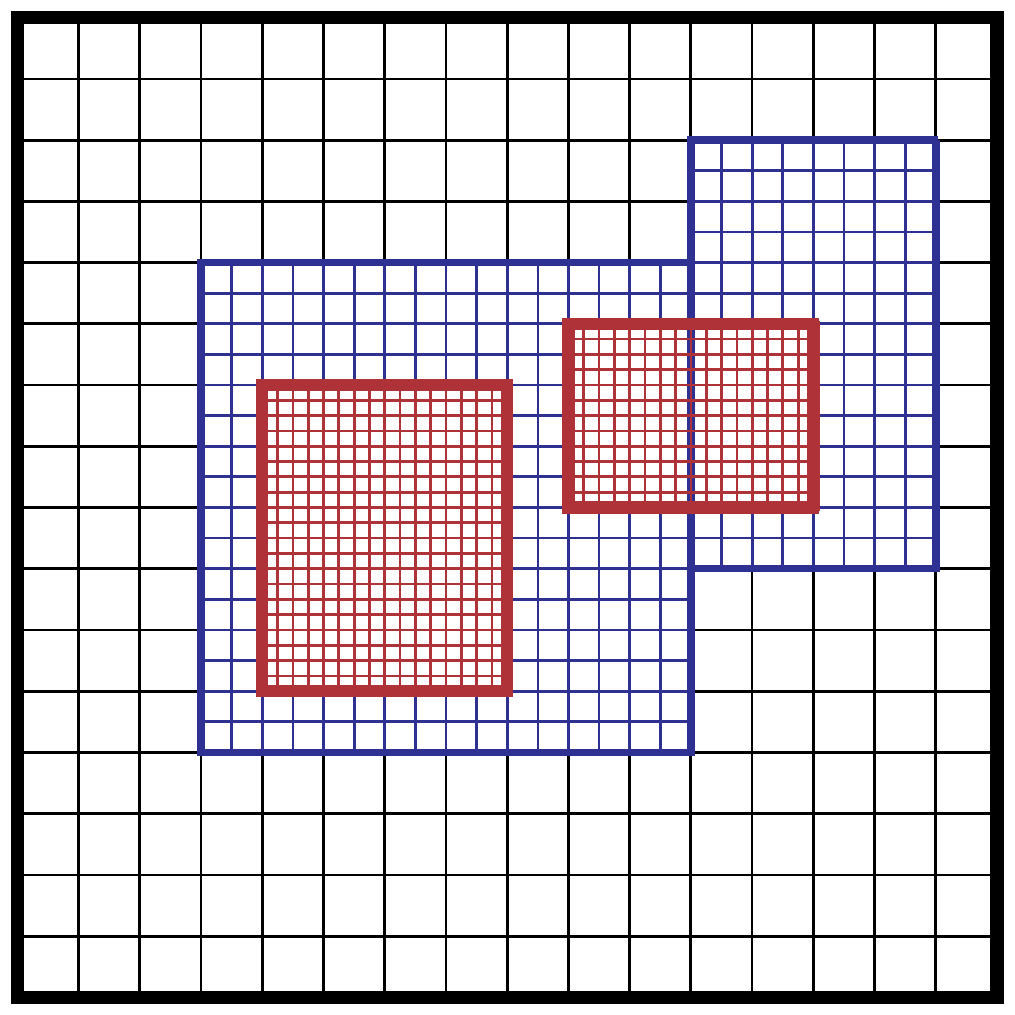
\includegraphics[width=3in]{./Basics/amrgrids.pdf}
  \caption{\label{fig:basics:amrgrids} Example of AMR grids.  There are
    three levels in total.}
\end{figure}

\section{Box, IntVect and IndexType}
\label{sec:basics:box}

{\tt Box} is the data structure for representing a rectangular domain
in indexing space.  For example, in Figure~\ref{fig:basics:amrgrids},
there are 1, 2 and 2 {\tt Box}es on levels 0, 1 and 2, respectively.
{\tt Box} is a dimension dependent class.  It has lower and upper
corners (represented by {\tt IntVect} and an index type (represented
by {\tt IndexType}).  There are no floating-point data in the object.

\subsection{IntVect}

{\idxamrex{IntVect}} is a dimension dependent class representing an
integer vector in {\idxamrex{AMREX\_SPACEDIM}}-dimensional space.  An
{\tt IntVect} can be constructed as follows,
\begin{lstlisting}[language=cpp]
 IntVect iv(AMREX_D_DECL(19, 0, 5));
\end{lstlisting}
Here {\tt AMREX\_D\_DECL} is a macro that expands {\tt
  AMREX\_D\_DECL(19,0,5)} to either {\tt 19} or {\tt 19,0} or {\tt
  19,0,5} depending on the number of dimensions.  The data can be
accessed via {\tt operator[]}, and the internal data pointer can be
returned by function {\tt getVect}.  For example
\begin{lstlisting}[language=cpp]
 for (int idim = 0; idim < AMREX_SPACEDIM; ++idim) {
     amrex::Print() << "iv[" << idim << "] = " << iv[idim] << "\n";
 }
 const int * p = iv.getVect();  // This can be passed to Fortran/C as an array
\end{lstlisting}

The class has a static function {\tt TheZeroVector()} returning the
zero vector, {\tt TheUnitVector()} returning the unit vector, and {\tt
  TheDimensionVector (int dir)} returning a reference to a constant
{\tt IntVect} that is zero except in the {\tt dir}-direction.  Note
the direction is zero-based.  {\tt IntVect} has a number of relational
operators, {\tt ==}, {\tt !=}, {\tt <}, {\tt <=}, {\tt >}, and {\tt
  >=} that can be used for lexicographical comparison (e.g., key of
{\tt std::map}), and a class {\tt IntVect::shift\_hasher} that can be
used as a hash function (e.g., for {\tt std::unordered\_map}).  It
also has various arithmetic operators.  For example,
\begin{lstlisting}[language=cpp]
 IntVect iv(AMREX_D_DECL(19, 0, 5));
 IntVect iv2((AMREX_D_DECL(4, 8, 0));
 iv += iv2;  // iv is now (23,8,5)
 iv *= 2;    // iv is now (46,16,10);
\end{lstlisting}

In AMR codes, one often needs to do refinement and coarsening on {\tt
  IntVect}.  The refinement operation can be done with the
multiplication operation.  However, the coarsening requires care
because of the rounding towards zero behavior of integer division in
Fortran, C and C++.  For example {\tt int i = -1/2} gives {\tt i =
  0}, and what we want is usually {\tt i = -1}.  Thus, one should use
the {\tt coarsen} functions:
\begin{lstlisting}[language=cpp]
  IntVect iv(AMREX_D_DECL(127,127,127));
  IntVect coarsening_ratio(AMREX_D_DECL(2,2,2));
  iv.coarsen(2);                 // Coarsen each component by 2
  iv.coarsen(coarsening_ratio);  // Component-wise coarsening
  const auto& iv2 = amrex::coarsen(iv, 2); // Return an IntVect w/o modifying iv
  IntVect iv3 = amrex::coarsen(iv, coarsening_return); // iv not modified
\end{lstlisting}

Finally, we note that {\tt operator<<} is overloaded for {\tt
  IntVect} and therefore one can call
\begin{lstlisting}[language=cpp]
  amrex::Print() << iv << "\n";
  std::cout << iv << "\n";
\end{lstlisting}

\subsection{IndexType}

This class defines an index as being cell based or node based in
each dimension.  The default constructor defines a cell based type in
all directions.  One can also construct an {\tt IndexType} with an
{\tt IntVect} with zero and one representing cell and node,
respectively.
\begin{lstlisting}[language=cpp]
 // Node in x-direction and cell based in y and z-directions
 // (i.e., x-face of numerical cells)
 IndexType xface(IntVect{AMREX_D_DECL(1,0,0)});
\end{lstlisting}
The class provides various functions including
\begin{lstlisting}[language=cpp]
 // True if the IndexType is cell based in all directions.
 bool cellCentered () const;

 // True if the IndexType is cell based in dir-direction.
 bool cellCentered (int dir) const;

 // True if the IndexType is node based in all directions.
 bool nodeCentered () const;

 // True if the IndexType is node based in dir-direction.
 bool nodeCentered (int dir) const;
\end{lstlisting}

Index type is a very important concept in \amrex.  It is a way of
representing the notion of indices $i$ and $i+1/2$.

\subsection{Box}

A {\tt Box} is an abstraction for defining discrete regions of {\tt
  AMREX\_SPACEDIM}-dimensional indexing space.  {\tt Box}es have an
{\tt IndexType} and two {\tt IntVect}s representing the lower and
upper corners.  Boxes can exist in positive and negative indexing
space.   Typical ways of defining a {\tt Box} are
\begin{lstlisting}[language=cpp]
 IntVect lo(AMREX_D_DECL(64,64,64));
 IntVect hi(AMREX_D_DECL(127,127,127));
 IndexType typ({AMREX_D_DECL(1,1,1)});
 Box cc(lo,hi);        // By default, Box is cell based.
 Box nd(lo,hi+1,typ);  // Construct a nodal Box.
 Print() << "A cell-centered Box " << cc << "\n";
 Print() << "An all nodal Box    " << nd << "\n";
\end{lstlisting}
Depending the dimensionality, the output of the code above is
\begin{verbatim}
  A cell-centered Box ((64,64,64) (127,127,127) (0,0,0))
  An all nodal Box    ((64,64,64) (128,128,128) (1,1,1))
\end{verbatim}
For simplicity, we will assume it is 3D for the rest of this section.
In the output, three integer tuples for each box are the lower corner
indices, upper corner indices, and the index types.  Note that {\tt 0}
and {\tt 1} denote cell and node, respectively.  For each tuple like
{\tt (64,64,64)}, the 3 numbers are for 3 directions.  The two {\tt
  Box}es in the code above represent different indexing views of the
same domain of $64^3$ cells.  Note that in \amrex\ convention, the
lower side of a cell has the same integer value as the cell centered
index.  That is if we consider a cell based index represent $i$, the
nodal index with the same integer value represents $i-1/2$.
Figure~\ref{fig:basics:indextypes} shows a 2D example of various index
types.  

\begin{figure}
  \centering
  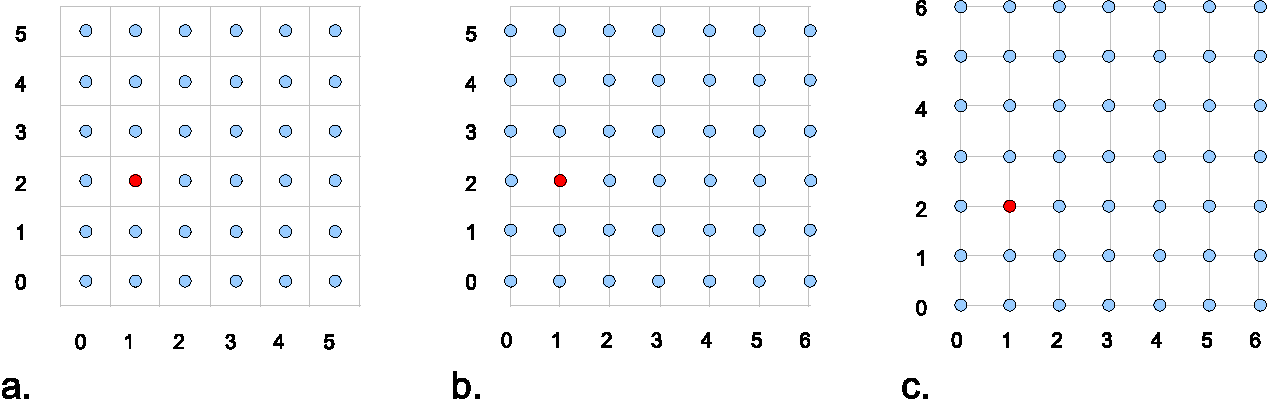
\includegraphics[width=5in]{./Basics/indextypes.pdf}
  \caption{\label{fig:basics:indextypes} Some of the different index
    types in two dimensions: (a) cell-centered, (b) face-centered,
    i.e., nodal in one dimensions ($x$) only, and (c) corner/nodal,
    i.e., nodal in all dimensions.  Note that for data that is nodal
    in one or more direction, the integer index corresponds to the
    lower boundary in that direction.}
\end{figure}

There are a number of ways of converting a {\tt Box} from one type to
another.
\begin{lstlisting}[language=cpp]
  Box b0 ({64,64,64}, {127,127}); // Index type: (cell, cell, cell)

  Box b1 = surroundingNodes(b0);  // A new Box with type (node, node, node)
  Print() << b1;                  // ((64,64,64) (128,128,128) (1,1,1))
  Print() << b0;                  // Still ((64,64,64) (127,127,127) (0,0,0))

  Box b2 = enclosedCells(b1);     // A new Box with type (node, node, node)
  if (b2 == b0) {                 // Yes, they are identical.
     Print() << "b0 and b2 are identical!\n";
  }

  Box b3 = convert(b0, {0,1,0});  // A new Box with type (cell, node, cell)
  Print() << b3;                  // ((64,64,64) (127,128,127) (0,1,0))

  b3.convert({0,0,1});            // Convert b0 to type (cell, cell, node)
  Print() << b3;                  // ((64,64,64) (127,127,128) (0,0,1))

  b3.surroundingNodes();          //  Exercise for you
  b3.enclosedCells();             //  Exercise for you
\end{lstlisting}

The internal data of {\tt Box} can be accessed via various member functions.
Examples are
\begin{lstlisting}[language=cpp]
  const IntVect& smallEnd () const&;  // Get the small end of the Box
  int bigEnd (int dir) const;         // Get the big end in dir direction
  const int* loVect () const&;        // Get a const pointer to the lower end
  const int* hiVect () const&;        // Get a const pointer to the upper end
\end{lstlisting}

{\tt Box}es can be refined and coarsened.  Refinement or coarsening
does not change the index type.  Some examples are shown below.
\begin{lstlisting}[language=cpp]
  Box ccbx ({16,16,16}, {31,31,31});
  ccbx.refine(2);
  Print() << ccbx;                   // ((32,32,32) (63,63,63) (0,0,0))
  Print() << ccbx.coarsen(2);        // ((16,16,16) (31,31,31) (0,0,0))

  Box ndbx ({16,16,16}, {32,32,32}, {1,1,1});
  ndbx.refine(2);
  Print() << ndbx;                   // ((32,32,32) (64,64,64) (1,1,1))
  Print() << ndbx.coarsen(2);        // ((16,16,16) (32,32,32) (1,1,1))

  Box facebx ({16,16,16}, {32,31,31}, {1,0,0});
  facebx.refine(2);
  Print() << facebx;                 // ((32,32,32) (64,63,63) (1,0,0))
  Print() << facebx.coarsen(2);      // ((16,16,16) (32,31,31) (1,0,0))

  Box uncoarsenable ({16,16,16}, {30,30,30});
  print() << uncoarsenable.coarsen(2); // ({8,8,8}, {15,15,15});
  print() << uncoarsenable.refine(2);  // ({16,16,16}, {31,31,31});
                                       // Different from the original!
\end{lstlisting}
Note that refinement and coarsening behaviors depend on the indexing
type.  One should think the refinement and coarsening in AMR context
that refined or coarsened {\tt Box} still covers the same physical
domain.  {\tt Box uncoarsenable} in the example above is considered
uncoarsenable because its coarsened version does not cover the same
physical domain in the AMR context.

{\tt Box}es can grow and they can grow in all directions or just one
direction.  There are a number of {\tt grow} functions.  Some are
member functions of the {\tt Box} class and others are non-member
functions in the {\tt amrex} namespace. 

{\tt Box} class provides the following member functions testing if a {\tt
  Box} or {\tt IntVect} is contained within this {\tt Box}.  Note that
it is a runtime error if the two {\tt Box}es have different types.
\begin{lstlisting}[language=cpp]
  bool contains (const Box& b) const;
  bool strictly_contains (const Box& b) const;
  bool contains (const IntVect& p) const;
  bool strictly_contains (const IntVect& p) const;
\end{lstlisting}

Another very common operation is the intersection of two {\tt Box}es
like in the following examples.
\begin{lstlisting}[language=cpp]
  Box b0 ({16,16,16}, {31,31,31});
  Box b1 ({ 0, 0,30}, {23,23,63});
  if (b0.intersects(b1)) {                  // true
      Print() << "b0 and b1 intersect.\n"; 
  }

  Box b2 = b0 & b1;     // b0 and b1 unchanged
  Print() << b2;        // ((16,16,30) (23,23,31) (0,0,0))

  Box b3 = surroundingNodes(b0) & surroundingNodes(b1); // b0 and b1 unchanged
  Print() << b3;        // ((16,16,30) (24,24,32) (1,1,1))

  b0 &= b2;             // b2 unchanged
  Print() << b0;        // ((16,16,30) (23,23,31) (0,0,0))

  b0 &= b3;             // Runtime error because of type mismatch!
\end{lstlisting}

\section{RealBox and Geometry}

A {\tt RealBox} stores the physical location in floating-point numbers
of the lower and upper corners of a rectangular domain.

{\tt Geometry} class describes problem domain and coordinate system
for rectangular problem domains.  A {\tt Geometry} object can be
constructed with
\begin{lstlisting}[language=cpp]
  explicit Geometry (const Box&     dom,
                     const RealBox* rb     = nullptr,
                     int            coord  = -1,
                     int*           is_per = nullptr);
\end{lstlisting}
Here the constructor takes a {\tt Box} specifying the indexing space
domain, an optional argument of {\tt RealBox} pointer specifying the
physical domain, an optional {\tt int} specifying coordinate system
type, and an optional {\tt int *} specifying periodicity.  If a {\tt
  RealBox} is not given, \amrex\ will construct one based on {\tt
  ParmParse} parameters, {\tt geometry.prob\_lo} and {\tt
  geometry.prob\_hi}, where each of the parameter is an array of {\tt
  AMREX\_SPACEDIM} real numbers.  It's a runtime error if this fails.
The optional argument for coordinate system is an integer type with
valid values being 0 (Cartesian), or 1 (cylindrical), or 2
(spherical).  If it is invalid as in the case of the default argument
value, \amrex\ will query the {\tt ParmParse} database for {\tt
  geometry.coord\_sys} and use it if one is found.  If it cannot find
the parameter, the coordinate system is set to 0 (i.e., Cartesian
coordinates).  {\tt Geometry} class has the concept of periodicity.
An optional argument can be passed specifying periodicity in each
dimension.  If it is not given, the domain is assumed to be
non-periodic unless there is the {\tt ParmParse} integer array
parameter {\tt geometry.is\_periodic} with {\tt 0} denoting
non-periodic and {\tt 1} denoting periodic.  Below is an example of
defining a {\tt Geometry} for a periodic rectangular domain of
$[-1.0,1.0]$ in each direction discretized with $64$ numerical cells
in each direction.
\begin{lstlisting}[language=cpp]
  int n_cell = 64;

  // This defines a Box with n_cell cells in each direction.
  Box domain(IntVect{AMREX_D_DECL(       0,        0,        0)},
             IntVect{AMREX_D_DECL(n_cell-1, n_cell-1, n_cell-1)});

  // This defines the physical box, [-1,1] in each direction.
  RealBox real_box({AMREX_D_DECL(-1.0,-1.0,-1.0)},
                   {AMREX_D_DECL( 1.0, 1.0, 1.0)});
  
  // This says we are using Cartesian coordinates
  int coord = 0;
  
  // This sets the boundary conditions to be doubly or triply periodic
  std::array<int,AMREX_SPACEDIM> is_periodic {AMREX_D_DECL(1,1,1)};
  
  // This defines a Geometry object
  Geometry geom(domain, &real_box, coord, is_periodic.data());
\end{lstlisting}

A {\tt Geometry} object can return various information of the physical
domain and the indexing space domain.  For example,
\begin{lstlisting}[language=cpp]
  const Real* problo = geom.ProbLo();  // Lower corner of the physical domain
  Real yhi = geom.ProbHi(1);           // y-direction upper corner
  const Real* dx = geom.CellSize();    // Cell size for each direction
  const Box& domain = geom.Domain();   // Index domain
  bool is_per = geom.isPeriodic(0);    // Is periodic in x-direction?
\end{lstlisting}


\section{BoxArray}
\label{sec:basics:ba}

{\tt BoxArray} is a class for storing a collection of {\tt Box}es on
a single AMR level.  One can make a {\tt BoxArray} out of a single {\tt Box}
and then chop it into multiple {\tt Box}es.
\begin{lstlisting}[language=cpp]
  Box domain(IntVect{0,0,0}, IntVect{127,127,127});
  BoxArray ba(domain);  // Make a new BoxArray out of a single Box
  Print() << "BoxArray size is " << ba.size() << "\n";  // 1
  ba.maxSize(64);       // Chop into boxes of 64^3 cells
  Print() << ba;
\end{lstlisting}
The output is like below,
\begin{verbatim}
  (BoxArray maxbox(8)
         m_ref->m_hash_sig(0)
  ((0,0,0) (63,63,63) (0,0,0)) ((64,0,0) (127,63,63) (0,0,0))
  ((0,64,0) (63,127,63) (0,0,0)) ((64,64,0) (127,127,63) (0,0,0))
  ((0,0,64) (63,63,127) (0,0,0)) ((64,0,64) (127,63,127) (0,0,0))
  ((0,64,64) (63,127,127) (0,0,0)) ((64,64,64) (127,127,127) (0,0,0)) )
\end{verbatim}
It shows that {\tt ba} now has 8 {\tt Box}es, and it also prints out
each {\tt Box}es.  

In \amrex, {\tt BoxArray} is a global data structure.  It holds all
the {\tt Box}es in a collection, even though a single process in a
parallel run only owns some of the {\tt Box}es via domain
decomposition.  In the example above, a 4-process run may divide the
work and each process owns say 2 {\tt Box}es
(Section~\ref{sec:basics:dm}).  Each process can then allocate memory
for the floating point data on the {\tt Box}es it owns
(Sections~\ref{sec:basics:multifab} \& \ref{sec:basics:fab}). 

{\tt BoxArray} has an indexing type, just like {\tt Box}.  Each {\tt
  Box} in a {\tt BoxArray} has the same type as the {\tt BoxArray}
itself.  In the following example, we show how one can convert {\tt
  BoxArray} to a different type. 
\begin{lstlisting}[language=cpp]
  BoxArray cellba(Box(IntVect{0,0,0}, IntVect{63,127,127}));
  cellba.maxSize(64);
  BoxArray faceba = cellba;
  // convert to index type (cell, cell, node)
  faceba.convert(IntVect{0,0,1});
  // Return an all node BoxArray
  const BoxArray& nodeba = amrex::convert(faceba, IntVect{1,1,1});
  Print() << cellba[0] << "\n";  // ((0,0,0) (63,63,63) (0,0,0))
  Print() << faceba[0] << "\n";  // ((0,0,0) (63,63,64) (0,0,1))  
  Print() << nodeba[0] << "\n";  // ((0,0,0) (64,64,64) (1,1,1))
\end{lstlisting}

As shown in the example above, {\tt BoxArray} has an {\tt operator[]}
that returns a {\tt Box} given an index.  It should be emphasized that
there is a difference between its behavior and the usual behavior of
an subscript operator one might expect.  The subscript operator in
{\tt BoxArray} returns by value instead of reference.  This means code
like below is meaningless because it modifies a temporary return
value. 
\begin{lstlisting}[language=cpp]
  ba[3].coarsen(2);  // DO NOT DO THIS!  Doesn't do what one might expect.
\end{lstlisting}

{\tt BoxArray} has a number of member functions that allow the {\tt
  Box}es to be modified.  For example,
\begin{lstlisting}[language=cpp]
  BoxArray& refine (int refinement_ratio);   // Refine each Box in BoxArray
  BoxArray& refine (const IntVect& refinement_ratio);
  BoxArray& coarsen (int refinement_ratio);  // Coarsen each Box in BoxArray
  BoxArray& coarsen (const IntVect& refinement_ratio);
\end{lstlisting}

We have mentioned at the beginning of this section that {\tt BoxArray}
is a global data structure storing {\tt Box}es owned by all processes.
The operation of deep copy is thus undesirable because the operation
itself is expensive and the extra copy wastes memory.  The
implementation of the {\tt BoxArray} class uses {\tt std::shared\_ptr}
to an internal container holding the actual {\tt Box} data.  Thus
making a copy of {\tt BoxArray} is a quite cheap operation.  The
conversion of types and coarsening are also cheap because they can
share the internal data with the original {\tt BoxArray}.  Function
{\tt refine} does create a new deep copy of the original data.  Also
note that a {\tt BoxArray} and its variant with a different type share
the same internal data is an implementation detail.  We discuss this
so that the users are aware of the performance and resource cost.
Conceptually we can think of them as completely independent of each
other.

For advanced users, \amrex\ provides functions performing the
intersection of a {\tt BoxArray} and a {\tt Box}.  These functions are
much faster than a naive implementation of performing intersection of
the {\tt Box} with each {\tt Box} in the {\tt BoxArray}.  If one needs
to perform those intersections, functions {\tt amrex::intersect}, {\tt
  BoxArray:: intersects} and {\tt BoxArray::intersections} should be
used.

\section{DistributionMapping}
\label{sec:basics:dm}

{\tt DistributionMapping} is a class describes which process owns the
data living on the domains specified by the {\tt Box}es in a {\tt
  BoxArray}.  Like {\tt BoxArray}, {\tt DistributionMapping} has an
element for each {\tt Box}, including the ones owned by other parallel
processes.  A way to construct a {\tt DistributionMapping} object
given a {\tt BoxArray} is as follows.
\begin{lstlisting}[language=cpp]
  DistributionMapping dm {ba};
\end{lstlisting}
Oftentimes what one needs is simply making a copy. 
\begin{lstlisting}[language=cpp]
  DistributionMapping dm {another_dm};
\end{lstlisting}
Note that this class is built using {\tt std::shared\_ptr}.  Thus
making a copy is relatively cheap in terms of performance and memory
resources.  This class has a subscript operator that returns the
process ID at a given index.

By default, {\tt DistributionMapping} uses an algorithm based on space
filling curve to determine distribution.  One can change the default
via {\tt ParmParse} paramter {\tt DistributionMapping.strategy}.  {\tt
  KNAPSACK} is a common choice that is optimized for load balance.
One can also explicitly construct a certain type of distribution.
{\tt DistributionMapping} class allows the user to have complete control by
passing an array of integers. 
\begin{lstlisting}[language=cpp]
  DistributionMapping dm;   // empty object
  Array<int> pmap;
  // The user fills the pmap array with the values specifying owner processes
  dm.define(pmap);  // Build DistributionMapping given an array of process IDs.
\end{lstlisting}


\section{BaseFab, FArrayBox and IArrayBox}
\label{sec:basics:fab}

\amrex\ is a block-structured AMR framework.  Although AMR introduces
irregularity to the data and algorithms, there is regularity at the
block/{\tt Box} level due to rectangular domain and the data structure
at the {\tt Box} level is conceptually simple.  {\tt BaseFab} is a
class template for multi-dimensional array-like data structure on a
{\tt Box}.  The template parameter is typically basic types such as
{\tt Real}, {\tt int} or {\tt char}.  The dimensionality of the array
is {\tt AMREX\_SPACEDIM} plus one.  The additional dimensional is for
the number of components.  The data are internally stored in a
contiguous block of memory in Fortran array order (i.e., column-major
order) for $(x,y,z,\mathrm{component})$, and each component also
occupies a contiguous block of memory because of the ordering.  For
example, a {\tt BaseFab<Real>} with 4 components defined on a
three-dimensional {\tt Box(IntVect\{-4,8,32\},IntVect\{32,64,48\})} is
like a Fortran array of {\tt real(amrex\_real),
  dimension(-4:32,8:64,32:48,0:3)}.  Note that the convention in \cpp\
part of \amrex\ is the component index is zero based.  The code for
constructing such an object is as follows,
\begin{lstlisting}[language=cpp]
  Box bx(IntVect{-4,8,32}, IntVect{32,64,48});
  int numcomps = 4;
  BaseFab<Real> fab(bx,numcomps);
\end{lstlisting}

Most applications do not use {\tt BaseFab} directly, but utilize
specialized classes derived from {\tt BaseFab}.  The most common types
are {\tt FArrayBox} derived from {\tt BaseFab<Real>} and {\tt
  IArrayBox} derived from {\tt BaseFab<int>}.

These derived classes also obtain many {\tt BaseFab} member functions
via inheritance.  We now show some common usages of these functions.
To get the {\tt Box} where a {\tt BaseFab} or its derived object is
defined, one can call
\begin{lstlisting}[language=cpp]
  const Box& box() const;
\end{lstlisting}
To the number of component, one can call
\begin{lstlisting}[language=cpp]
  int nComp() const;
\end{lstlisting}
To get a pointer to the array data, one can call
\begin{lstlisting}[language=cpp]
  T* dataPtr(int n=0);     // Data pointer to the nth component
                           // T is template parameter (e.g., Real)
  const T* dataPtr(int n=0) const; // const version
\end{lstlisting}
The typical usage of the returned pointer is then to pass it to a
Fortran or C function that works on the array data (see
Section~\ref{sec:basics:fortran}).
{\tt BaseFab} has several functions that set the array data to a
constant value (e.g., 0).  Two examples are as follows.  
\begin{lstlisting}[language=cpp]
  void setVal(T x);        // Set all data to x
  // Set the sub-region specified by bx to value x starting from component
  // nstart.  ncomp is the total number of component to be set.
  void setVal(T x, const Box& bx, int nstart, int ncomp);
\end{lstlisting}
One can copy data from one {\tt BaseFab} to another.
\begin{lstlisting}[language=cpp]
  BaseFab<T>& copy (const BaseFab<T>& src, const Box& srcbox, int srccomp,
                    const Box& destbox, int destcomp, int numcomp);
\end{lstlisting}
Here the function copies the data from the region specified by {\tt
  srcbox} in the source {\tt BaseFab src} into the region specified by
{\tt destbox} in the destination {\tt BaseFab} that invokes the
function.  Note that although {\tt srcbox} and {\tt destbox} may be
different, they must be the same size and shape, otherwise a runtime
error occurs.  The user also specifies how many components ({\tt int
  numcomp}) are copied starting at component {\tt srccomp} in {\tt
  src} and stored starting at component {\tt destcomp}.  {\tt BaseFab}
has functions returning the minimum or maximum value.
\begin{lstlisting}[language=cpp] 
  T min (int comp=0) const;  // Minimum value of given component.
  T min (const Box& subbox, int comp=0) const; // Minimum value of given 
                                               // component in given subbox.
  T max (int comp=0) const;  // Maximum value of given component.
  T max (const Box& subbox, int comp=0) const; // Maximum value of given 
                                               // component in given subbox.
\end{lstlisting}

{\tt BaseFab} also has many arithmetic functions.  Here are some
examples using {\tt FArrayBox}.
\begin{lstlisting}[language=cpp]
  Box box(IntVect{0,0,0}, IntVect{63,63,63});
  int ncomp = 2;
  FArrayBox fab1(box, ncomp);
  FArrayBox fab2(box, ncomp);
  fab1.setVal(1.0);    // Fill fab1 with 1.0
  fab1.mult(10.0, 0);  // Multiply component 0 by 10.0
  fab2.setVal(2.0);    // Fill fab2 with 2.0
  Real a = 3.0;
  fab2.saxpy(a, fab1); // For both components, fab2 <- a * fab1 + fab2
\end{lstlisting}
For more complicated expressions that not supported, one can write
Fortran or C functions for those (Section~\ref{sec:basics:fortran}).
Note that {\tt BaseFab} does provide operators for accessing the
data directly in \cpp.  For example, the {\tt saxpy} example above can
be done with
\begin{lstlisting}[language=cpp]
  // Iterate over all components
  for (int icomp=0; icomp < fab1.nComp(); ++icomp) {
      // Iterate over all cells in Box
      for (BoxIterator bit(fab1.box()); bit.ok(); ++bit) {
          // bit() returns IntVect
          fab2(bit(),icomp) = a * fab1(bit(),icomp) + fab2(bit(),icomp);
      }
  }
\end{lstlisting}
But this approach is generally not recommended for performance reason.
However, it can be handy for debugging.

{\tt BaseFab} and its derived classes are containers data on {\tt
  Box}.  We recall that {\tt Box} has types
(Section~\ref{sec:basics:box}).  The examples in this section so far
use the default cell based type.  However, some functions will result
in a runtime error if the types mismatch.  For example.
\begin{lstlisting}[language=cpp]
  Box ccbx ({16,16,16}, {31,31,31});           // cell centered box
  Box ndbx ({16,16,16}, {31,31,31}, {1,1,1});  // nodal box
  FArrayBox ccfab(ccbx);
  FArrayBox ndfab(ndbx);
  ccfab.setVal(0.0);
  ndfab.copy(ccfab);   // runtime error due to type mismatch
\end{lstlisting}

Because it typically contains a lot of data, {\tt BaseFab}'s copy
constructor and copy assignment operator are disabled for performance
reason.  However, it does provide a move constructor.  In addition, it
also provides a constructor for making an alias of an existing
object.  Here is an example using {\tt FArrayBox}.
\begin{lstlisting}[language=cpp]
  FArrayBox orig_fab(box, 4);  // 4-component FArrayBox
  // Make a 2-component FArrayBox that is an alias of rhs
  // starting from component 1.
  FArrayBox alias_fab(rhs, amrex::make_alias, 1, 2);
\end{lstlisting}
In the example, the alias {\tt FArrayBox} has only two components even
though the original one has four components.  The alias has a sliced
component view of the original {\tt FArrayBox}.  This is possible
because of the array ordering.  It is however not possible to slice in
the real space (i.e., the first {\tt AMREX\_SPACEDIM} dimensions).
Note that no new memory is allocated in constructing the alias and the
alias contains a non-owning pointer.  It should be emphasized that the
alias will contain a dangling pointer after the original {\tt
  FArrayBox} reaches its end of life.

\section{FabArray, MultiFab and iMultiFab}
\label{sec:basics:multifab}

{\tt FabArray<FAB>} is a class template for a collection of {\tt FAB}s
on the same AMR level associated with a {\tt BoxArray}
(Section~\ref{sec:basics:ba}).  The template parameter {\tt FAB} is
usually {\tt BaseFab<T>} or its derived classes (e.g., {\tt
  FArrayBox}).  However, it can also be used to hold other data
structures.  To construct a {\tt FabArray}, a {\tt BoxArray} must be
provided because it is intended to hold {\emph{grid}} data defined on
a union of rectangular regions embedded in a uniform index space.  For
example, an {\tt FabArray} object can be used to hold data for one
level of the example grids of Figure~\ref{fig:basics:amrgrids}.  The
{\tt BoxArray} on level 2 ({\emph{red}) has two {\tt Box}es.

{\tt FabArray} is a parallel data structure that the data (i.e.,
{\tt FAB}) are distributed among parallel processes.  On each process,
the {\tt FabArray} contains only the {\tt FAB} objects owned by this
process, and the process operates only on its local data.  For
operations that require data owned by other processes, remote
communications are involved.  Thus, the construction of a {\tt
  FabArray} requires a {\tt DistributionMapping}
(Section~\ref{sec:basics:dm}) that specifies which process owns which
{\tt Box}.  For level 2 ({\emph{red}) in
Figure~\ref{fig:basics:amrgrids}, there are two {\tt Box}es.  Suppose
there are two parallel processes, and we use a {\tt
  DistributionMapping} that assigns one {\tt Box} to each process.
For {\tt FabArray} on each process, it is built on a {\tt BoxArray} with
2 {\tt Box}es, but contains only one {\tt FAB}.  

In \amrex, there are some specialized classes derived from {\tt
  FabArray}.  The {\tt iMultiFab} class is derived from {\tt
  FabArray<IArrayBox>}.  The most commonly used {\tt FabArray} kind
class is {\tt MultiFab} derived from {\tt FabArray<FArrayBox>}.  In
the rest of this section, we use {\tt MultiFab} as example.  However,
these concepts are equally applicable to other types of {\tt
  FabArray}s.  There are many ways to define a {\tt MultiFab}.  For
example,
\begin{lstlisting}[language=cpp]
  // ba is BoxArray
  // dm is DistributionMapping
  int ncomp = 4;
  int ngrow = 1;
  MultiFab mf(ba, mf, ncomp, ngrow);
\end{lstlisting}
Here we define a {\tt MultiFab} with 4 components and 1 ghost cell.  A
{\tt MultiFab} contains a number of {\tt FArrayBox}es
(Section~\ref{sec:basics:fab}) defined on {\tt Box}es grown by the
number of ghost cells (1 in this example).  That is the {\tt Box} in
the {\tt FArrayBox} is not exactly the same as in the {\tt BoxArray}.
If the {\tt BoxArray} has a {\tt Box\{(8,8,8) (15,15,15)\}}, the one
used for constructing {\tt FArrayBox} will be {\tt Box\{(7,7,7)
  (16,16,16)\}} in this example.  Note that {\tt FArrayBox} itself
does not have the concept of ghost cell, whereas ghost cell is a key
concept of {\tt MultiFab} that allows for local operations on ghost
cell data originated from remote processes.  We will discuss how to
fill ghost cells later in this section.  {\tt MultiFab} also has a
default constructor.  One can define an empty {\tt MultiFab} first and
then call the {\tt define} function as follows.
\begin{lstlisting}[language=cpp]
  MultiFab mf;
  // ba is BoxArray
  // dm is DistributionMapping
  int ncomp = 4;
  int ngrow = 1;
  mf.define(ba, mf, ncomp, ngrow);
\end{lstlisting}
Given an existing {\tt MultiFab}, one can also make an alias {\tt
  MultiFab} as follows.
\begin{lstlisting}[language=cpp]
  // orig_mf is an existing Multifab
  int start_comp = 3;
  int num_comps = 1;
  MultiFab alias_mf(orig_mf, amrex::make_alias, start_comp, num_comps);
\end{lstlisting}
Here the first integer parameter is the starting component in the
original {\tt MultiFab} that will become component 0 in the alias {\tt
  MultiFab} and the second integer parameter is the number of
components in the alias.  It's a runtime error if the sum of the two
integer parameters is greater than the number of the components in the
original {\tt MultiFab}.  Note that the alias {\tt MultiFab} has
exactly the same number of ghost cells as the original {\tt MultiFab}.

We often need to build new {\tt MultiFab}s that have the same {\tt
  BoxArray} and {\tt DistributionMapping} as a given {\tt MultiFab}.
Below is an example of how to achieve this.
\begin{lstlisting}[language=cpp]
  // mf0 is an already defined MultiFab
  const BoxArray& ba = mf0.boxArray();
  const DistributionMapping& dm = mf0.DistributionMap();
  int ncomp = mf0.nComp();
  int ngrow = mf0.ngrow();
  MultiFab mf1(ba,dm,ncomp,ngrow);  // new MF with the same ncomp and ngrow
  MultiFab mf2(ba,dm,ncomp,0);      // new MF with no ghost cells
  // new MF with 1 component and 2 ghost cells
  MultiFab mf3(mf0.boxArray(), mf0.DistributionMap(), 1, 2);               
\end{lstlisting}

As we have repeatedly mentioned in this chapter that {\tt Box} and
{\tt BoxArray} have various index types.  Thus, {\tt MultiFab} also
has an index type that is obtained from the {\tt BoxArray} used for
defining the {\tt MultiFab}.  It should be noted again that index type
is a very important concept in \amrex.  Let's consider an example of a
finite-volume code, in which the state is defined as cell averaged
variables and the fluxes are defined as face averaged variables.
\begin{lstlisting}[language=cpp]
  // ba is cell-centered BoxArray
  // dm is DistributionMap
  int ncomp = 3;  // Suppose the system has 3 components
  int ngrow = 0;  // no ghost cells
  MultiFab state(ba, dm, ncomp, ngrow);
  MultiFab xflux(amrex::convert(ba, IntVect{1,0,0}), dm, ncomp, 0);
  MultiFab yflux(amrex::convert(ba, IntVect{0,1,0}), dm, ncomp, 0);
  MultiFab zflux(amrex::convert(ba, IntVect{0,0,1}), dm, ncomp, 0);
\end{lstlisting}
Here all {\tt MultiFab} use the same {\tt DistributionMapping}, but
their {\tt BoxArray}s have different.  The state is cell based,
whereas the fluxes are on the faces.  Suppose the cell based {\tt
  BoxArray} contains a {\tt Box\{(8,8,16), (15,15,31)\}}.  The state
on that {\tt Box} is conceptually a Fortran Array with the dimension
of {\tt (8:15,8:15,16:31,0:2)}.  The fluxes are arrays with slightly
different indices.  For example, the $x$-direction flux for that {\tt
  Box} has the dimension of {\tt (8:16,8:15,16:31,0:2)}.  Note there is
an extra element in $x$-direction.  


% common operations like Copy, Add, etc.

%ghost cells We note that while the grids themselves are 
%non-intersecting boxes, the data in an FArrayBox may be defined
%on a Box larger than the grid if ghost (or halo) cells are needed.
%
% parallel communication

\section{MFIter and Tiling}
\label{sec:basics:mfiter}

\section{Calling Fortan or C}
\label{sec:basics:fortran}

\section{Physical Boundary}

\section{I/O}

\section{Memory Allocation}

% resize

\section{Abort, Assertion, Floating-Point Exceptions, and Backtrace}
% FArrayBox init nan check nan .... contains_nan


\chapter{{\tt AmrCore} Source Code}\label{Chap:AmrCore}
On AmrCore



\chapter{{\tt Amr} Source Code}\label{Chap:AmrLevel}
AmrLevel class


\chapter{Particles}\label{Chap:Particles}
On particle


\chapter{Fortran Interface}\label{Chap:Fortran}
\input{Fortran/Fortran}

\chapter{Visualization}\label{Chap:Visualization}
There are several visualization tools that can be used for \amrex\
plotfiles.  The popular \visit\ package supports the \amrex\ file 
format natively (using the {\sf BoxLib2d} and {\sf BoxLib3d} file types),
as does the \yt\ python package.  The standard tool used within the
\amrex-community is \amrvis, a package developed and supported 
by CCSE that is designed specifically for highly efficient visualization
of block-structured hierarchical AMR data.

\section{\amrvis}

Our favorite visualization tool is \amrvis. We heartily encourage you
to build the {\tt amrvis2d} and {\tt amrvis3d} executables, and to try using them
to visualize your data. A very useful feature is View/Dataset, which
allows you to actually view the numbers in a spreadsheet that is nested
to reflect the AMR hierarchy -- this can be handy for
debugging. You can modify how many levels of data you want to see,
whether you want to see the grid boxes or not, what palette you use,
etc.  Here are some instructions and tips for using \amrvis:

\begin{enumerate}

\item Download and build \amrvis:
\begin{verbatim}
git clone https://ccse.lbl.gov/pub/Downloads/Amrvis.git
\end{verbatim}

Then {\tt cd} into {\tt Amrvis/}, edit the {\tt GNUmakefile} by
setting {\tt COMP} to the compiler suite you have.

Type {\tt make DIM=2} or {\tt make DIM=3} to build, 
resulting in an executable that looks like {\tt amrvis2d...ex}.

If you want to build amrvis with {\tt DIM=3}, you must first
download and build {\tt volpack}:
\begin{verbatim}
git clone https://ccse.lbl.gov/pub/Downloads/volpack.git
\end{verbatim}

Then {\tt cd} into {\tt volpack/} and type {\tt make}.

Note: \amrvis\ requires the OSF/Motif libraries and headers. If you don't have these 
you will need to install the development version of motif through your package manager. 
{\tt lesstif} gives some functionality and will allow you to build the amrvis executable, 
but \amrvis\ may exhibit subtle anomalies.

On most Linux distributions, the motif library is provided by the
{\tt openmotif} package, and its header files (like {\tt Xm.h}) are provided
by {\tt openmotif-devel}. If those packages are not installed, then use the
OS-specific package management tool to install them. 

You may then want to create an alias to {\tt amrvis2d}, for example
\begin{verbatim}
alias amrvis2d /tmp/Amrvis/amrvis2d...ex
\end{verbatim}

\item Run the command {\tt cp Amrvis/amrvis.defaults \textasciitilde/.amrvis.defaults}.
Then, in your copy, edit the line containing ``{\tt palette}'' line to point to, e.g., 
``{\tt palette  /home/username/Amrvis/Palette}''.  The other lines control
options such as the initial field to display, the number format, widow size, etc.
If there are multiple instances of the same option, the last option takes precedence.

\item Generally the plotfiles have the form {\tt pltXXXXX} 
  (the {\tt plt} prefix can be changed), where {\tt XXXXX} is a number 
  corresponding to the timestep the file
  was output.  {\tt amrvis2d <filename>} or {\tt amrvis3d <filename>}
  to see a single plotfile, 
  or for 2D data sets, {\tt amrvis2d -a plt*}, which will animate the 
  sequence of plotfiles.

  You can use the ``Variable'' menu to change the variable.
  You can left-click drag a box around a region
  and click "View'' $\rightarrow$ ``Dataset''
  in order to look at the actual numerical values
  (see Figure \ref{Fig:Amrvis}).
  Or you can simply left click on a point to obtain the numerical value.
  You can also export the
  pictures in several different formats under "File/Export".
  In 2D you can right and center click to get line-out plots.
  In 3D you can right and center click to change the planes, and the hold
  shift+(right or center) click to get line-out plots.

\begin{figure}[tb]
\centering
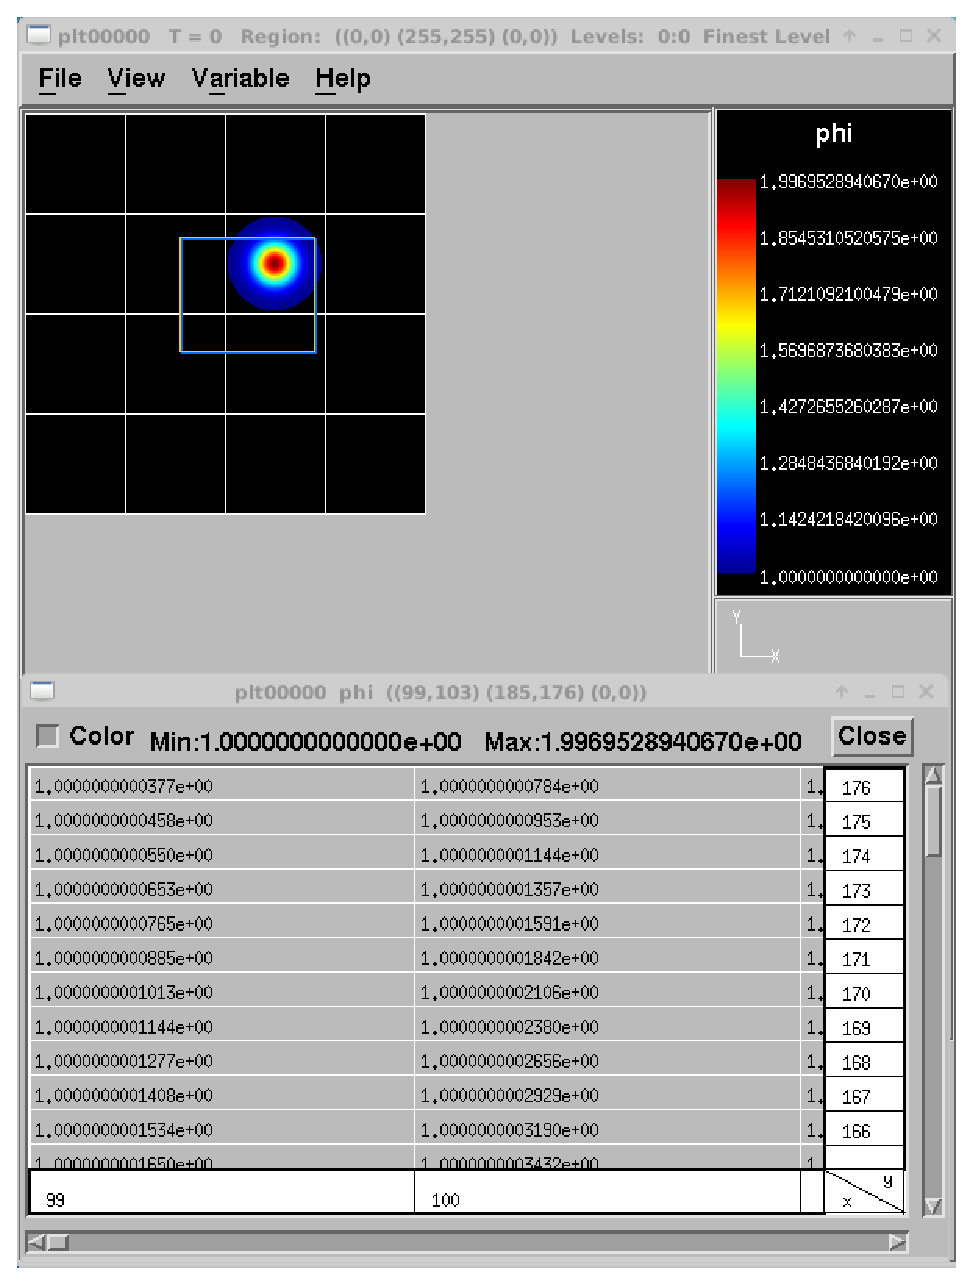
\includegraphics[width=2.5in]{./Visualization/Amrvis_2d}
~~~
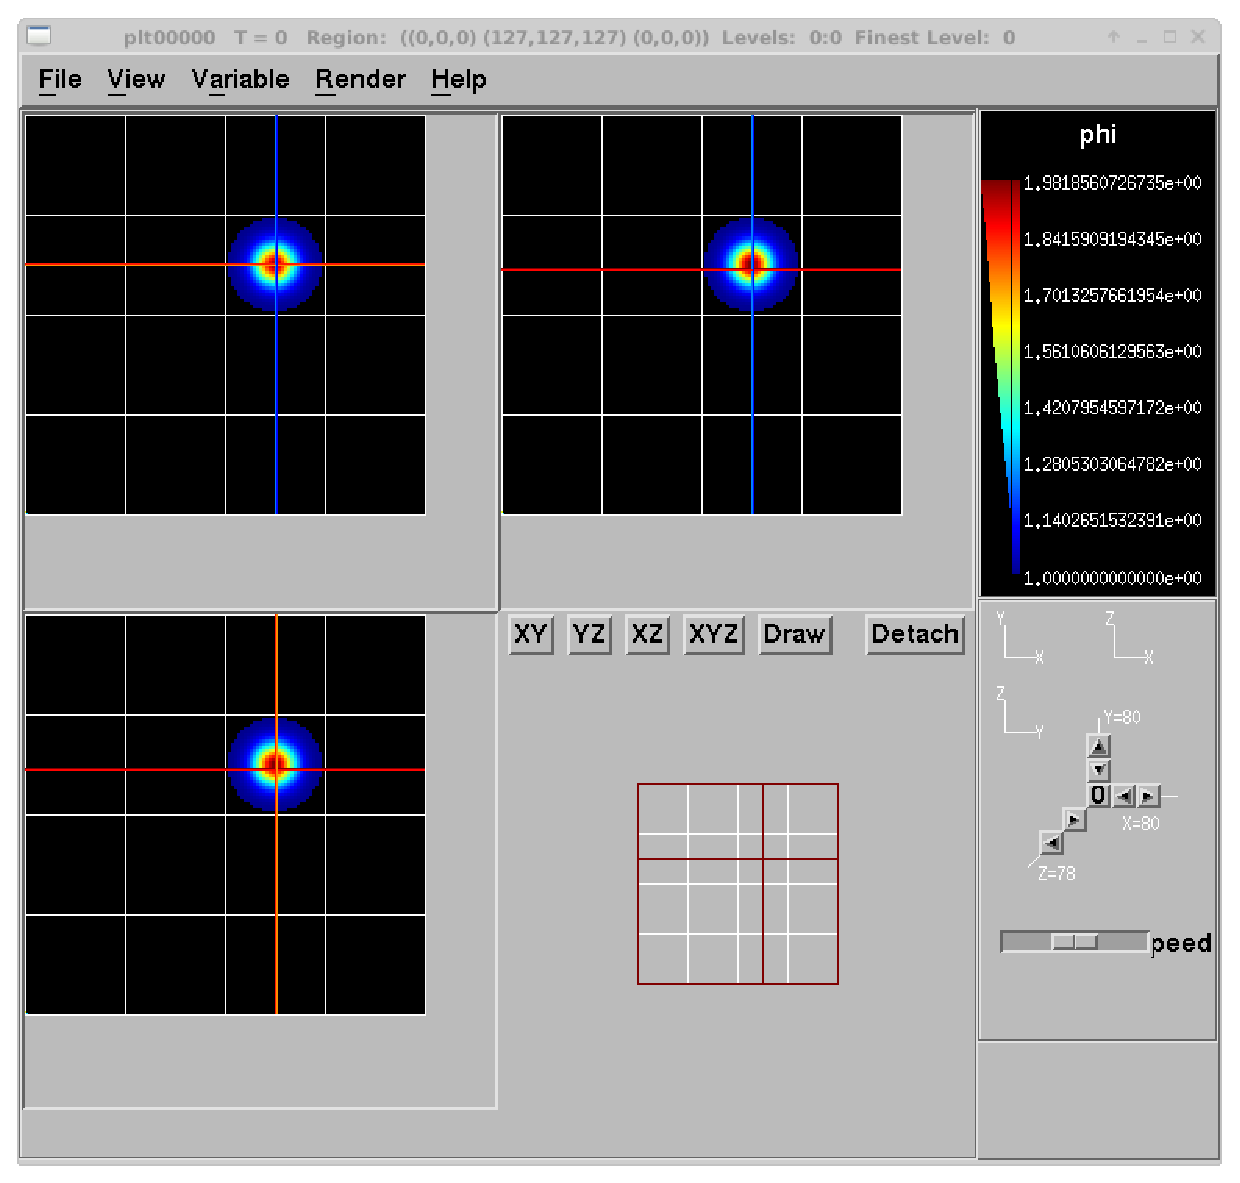
\includegraphics[width=2.5in]{./Visualization/Amrvis_3d}
\caption{2D and 3D images generated with Amrvis}
\label{Fig:Amrvis}
\end{figure}

  We have created a number of routines to convert \amrex\ plotfile data
  other formats (such as MATLAB), but in order to properly interpret 
  the hierarchical AMR data, each tends to have its own idiosyncrasies.
  If you would like to display the data in another format, please contact
  Marc Day ({\tt MSDay@lbl.gov}) and we will point you to whatever we have
  that can help.

\end{enumerate}

\section{\visit}
\label{sec:visit}

\amrex\ data can also be visualized by {\tt VisIt}, an open
source visualization and analysis software.  To follow along with this example,
first build and run the first heat equation tutorial code
(see Section \ref{sec:heat equation}).

Next, download and install {\tt VisIt} from \url{https://wci.llnl.gov/simulation/computer-codes/visit}.
To open a single plotfile, run {\tt VisIt}, then select ``File'' $\rightarrow$ ``Open file ...'',
then select the {\tt Header} file associated the the plotfile of interest (e.g., {\tt plt00000/Header}).
Assuming you ran the simulation in 2D, here are instructions for making a simple plot:
\begin{itemize}
\item To view the data, select ``Add'' $\rightarrow$ ``Pseudocolor'' $\rightarrow$ ``phi'', and then select
``Draw''.
\item To view the grid structure (not particularly interesting yet, but when we add AMR it will be), select
`` $\rightarrow$ ``subset'' $\rightarrow$ ``levels''.  Then double-click the text ``Subset - levels'',
enable the ``Wireframe'' option, select ``Apply'', select ``Dismiss'', and then select ``Draw''.
\item To save the image, select ``File'' $\rightarrow$ ``Set save options'', then customize the image format
to your liking, then click ``Save''.
\end{itemize}
Your image should look similar to the left side of Figure \ref{Fig:VisIt}.\\
\begin{figure}[tb]
\centering
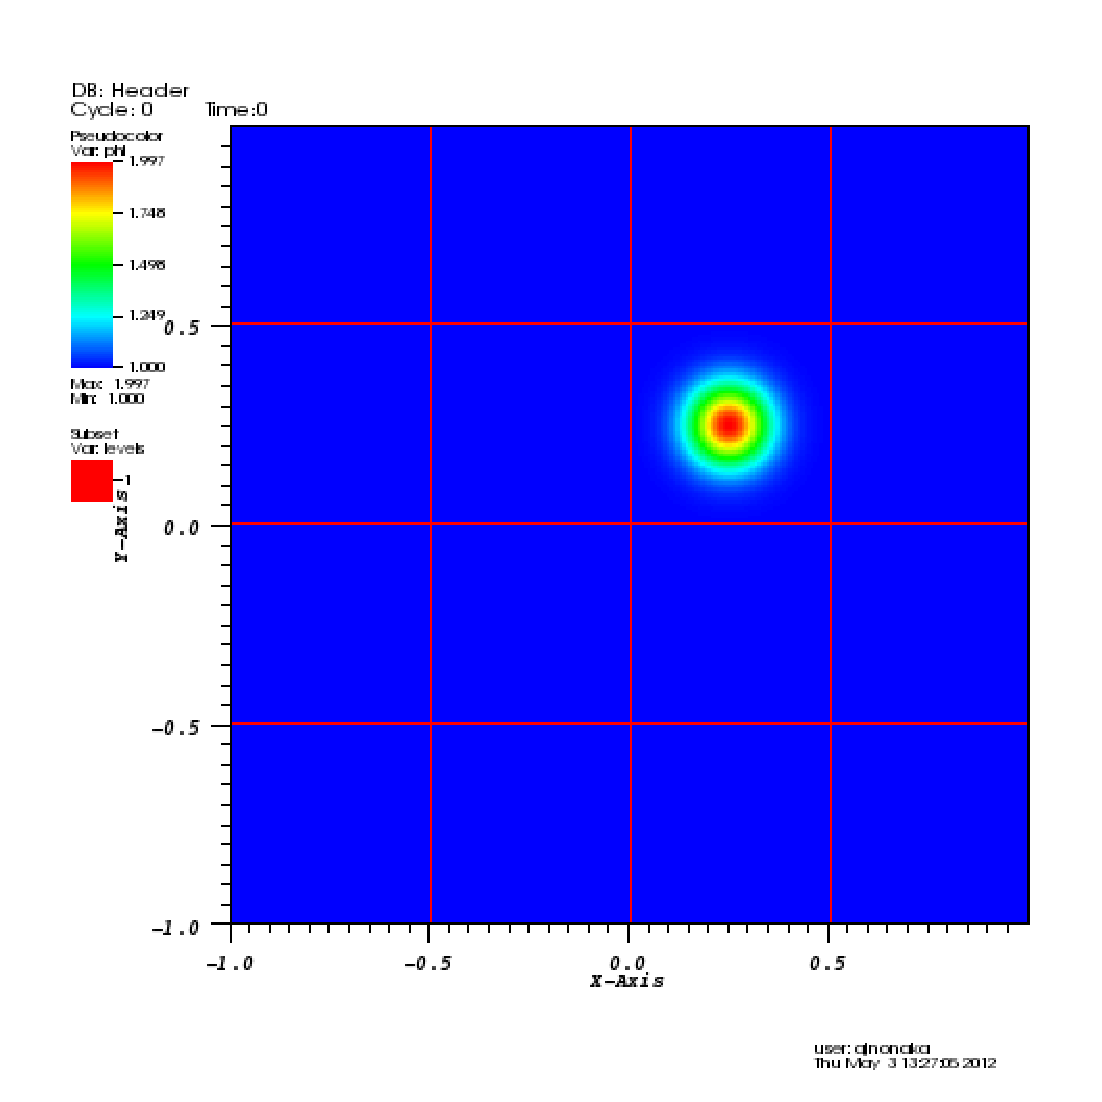
\includegraphics[width=3.1in]{./Visualization/VisIt_2D}
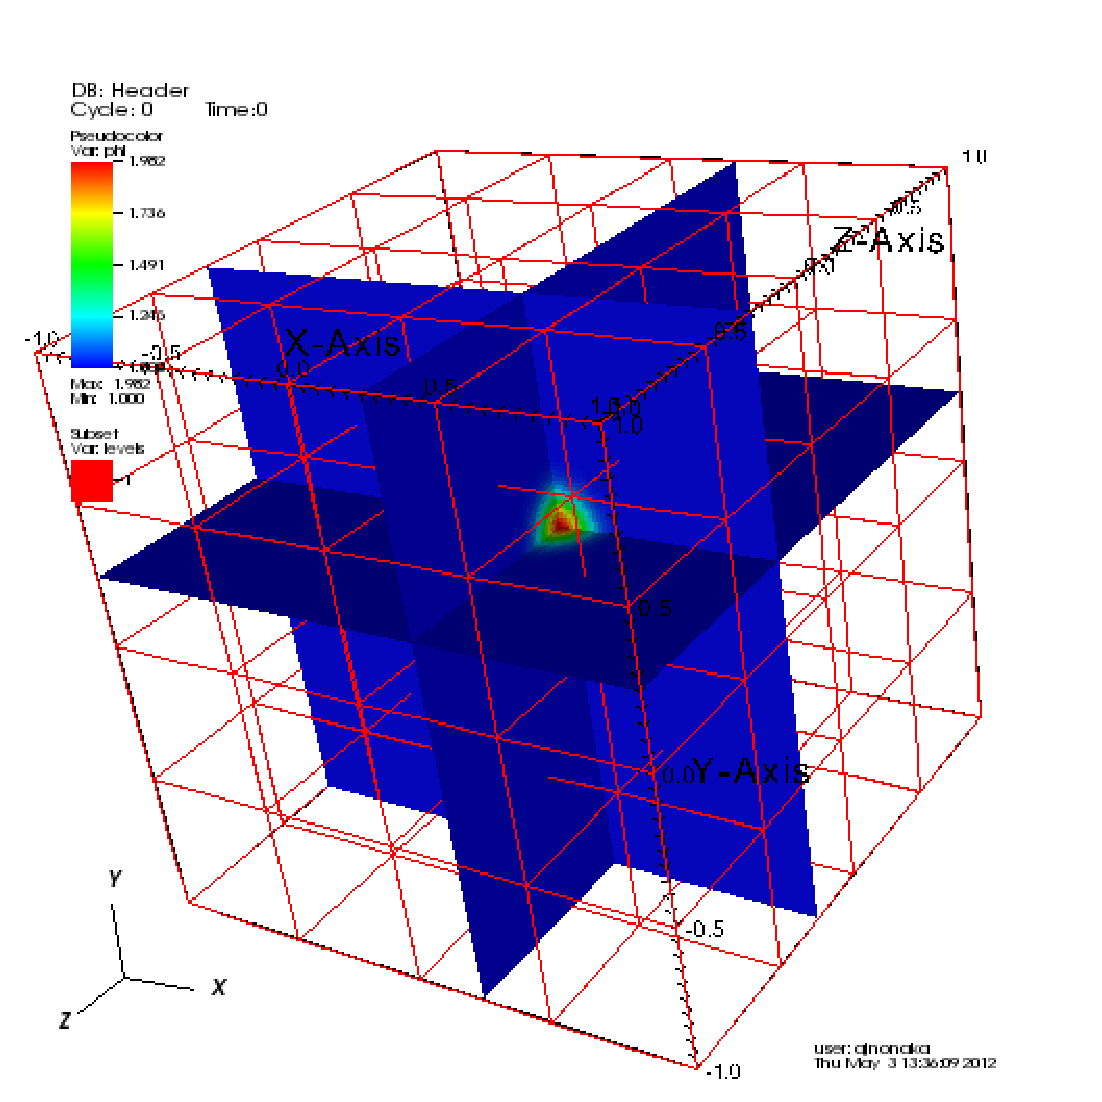
\includegraphics[width=3.1in]{./Visualization/VisIt_3D}
\caption{(Left) 2D image generated with VisIt.  (Right) 3D image generated with VisIt.}
\label{Fig:VisIt}
\end{figure}

In 3D, you must apply the ``Operators'' $\rightarrow$ ``Slicing'' $\rightarrow$ ``ThreeSlice'', with the 
``ThreeSlice operator attribute'' set to x=0.25, y=0.25, and z=0.25.  You can left-click and drag
over the image to rotate the image to generate something similar to right side of Figure \ref{Fig:VisIt}.\\

To make a movie, you must first create a text file named {\tt movie.visit} with a list of the {\tt Header} 
files for the individual frames.  This can most easily be done using the command:
\begin{lstlisting}[backgroundcolor=\color{light-red}]
~/amrex/Tutorials/Basic/HeatEquation_EX1_C> ls -1 plt*/Header | tee movie.visit
plt00000/Header
plt01000/Header
plt02000/Header
plt03000/Header
plt04000/Header
plt05000/Header
plt06000/Header
plt07000/Header
plt08000/Header
plt09000/Header
plt10000/Header
\end{lstlisting}
The next step is to run {\tt VisIt}, select ``File'' $\rightarrow$ ``Open file ...'',
then select {\tt movie.visit}.  Create an image to your liking and press the ``play'' button
on the VCR-like control panel to preview all the frames.  To save the movie, choose
``File'' $\rightarrow$ ``Save movie ...'', and follow the on-screen instructions.

\section{\yt}

\yt, an open source Python package available at \url{http://yt-project.org/},
can be used for analyzing and visualizing mesh and particle data generated by
\amrex\ codes.  Some of the \amrex\ developers are also \yt\ project members.
Below we describe how to use \yt\ on both a local workstation, as well as at
the NERSC HPC facility for high-throughput visualization of large data sets.

\subsection{Using \yt\ on a local workstation}

Running \yt\ on a local system generally provides good interactivity, but
limited performance. Consequently, this configuration is best when doing
exploratory visualization (e.g., experimenting with camera angles, lighting,
and color schemes) of small data sets.

To use \yt\ on an \amrex\ plot file, first start a Jupyter notebook or an IPython kernel, and import the \texttt{yt} module:

\begin{lstlisting}[language=python,breaklines=true]
In [1]: import yt

In [2]: print(yt.__version__)
3.4-dev
\end{lstlisting}

Next, load a plot file; in this example we use a plot file from the Nyx cosmology application:

\begin{lstlisting}[language=python,breaklines=true]
In [3]: ds = yt.load("plt00401")
yt : [INFO     ] 2017-05-23 10:03:56,182 Parameters: current_time              = 0.00605694344696544
yt : [INFO     ] 2017-05-23 10:03:56,182 Parameters: domain_dimensions         = [128 128 128]
yt : [INFO     ] 2017-05-23 10:03:56,182 Parameters: domain_left_edge          = [ 0.  0.  0.]
yt : [INFO     ] 2017-05-23 10:03:56,183 Parameters: domain_right_edge         = [ 14.24501  14.24501  14.24501]

In [4]: ds.field_list
Out[4]:
[('DM', 'particle_mass'),
 ('DM', 'particle_position_x'),
 ('DM', 'particle_position_y'),
 ('DM', 'particle_position_z'),
 ('DM', 'particle_velocity_x'),
 ('DM', 'particle_velocity_y'),
 ('DM', 'particle_velocity_z'),
 ('all', 'particle_mass'),
 ('all', 'particle_position_x'),
 ('all', 'particle_position_y'),
 ('all', 'particle_position_z'),
 ('all', 'particle_velocity_x'),
 ('all', 'particle_velocity_y'),
 ('all', 'particle_velocity_z'),
 ('boxlib', 'density'),
 ('boxlib', 'particle_mass_density')]
\end{lstlisting}

From here one can make slice plots, 3-D volume renderings, etc. An example of
the slice plot feature is shown below:

\begin{lstlisting}[language=python,breaklines=true]
In [9]: slc = yt.SlicePlot(ds, "z", "density")
yt : [INFO     ] 2017-05-23 10:08:25,358 xlim = 0.000000 14.245010
yt : [INFO     ] 2017-05-23 10:08:25,358 ylim = 0.000000 14.245010
yt : [INFO     ] 2017-05-23 10:08:25,359 xlim = 0.000000 14.245010
yt : [INFO     ] 2017-05-23 10:08:25,359 ylim = 0.000000 14.245010

In [10]: slc.show()

In [11]: slc.save()
yt : [INFO     ] 2017-05-23 10:08:34,021 Saving plot plt00401_Slice_z_density.png
Out[11]: ['plt00401_Slice_z_density.png']
\end{lstlisting}

The resulting image is Figure~\ref{fig:yt_Nyx_slice_plot}. One can also make
volume renderings with \yt; an example is show below:

\begin{figure}
  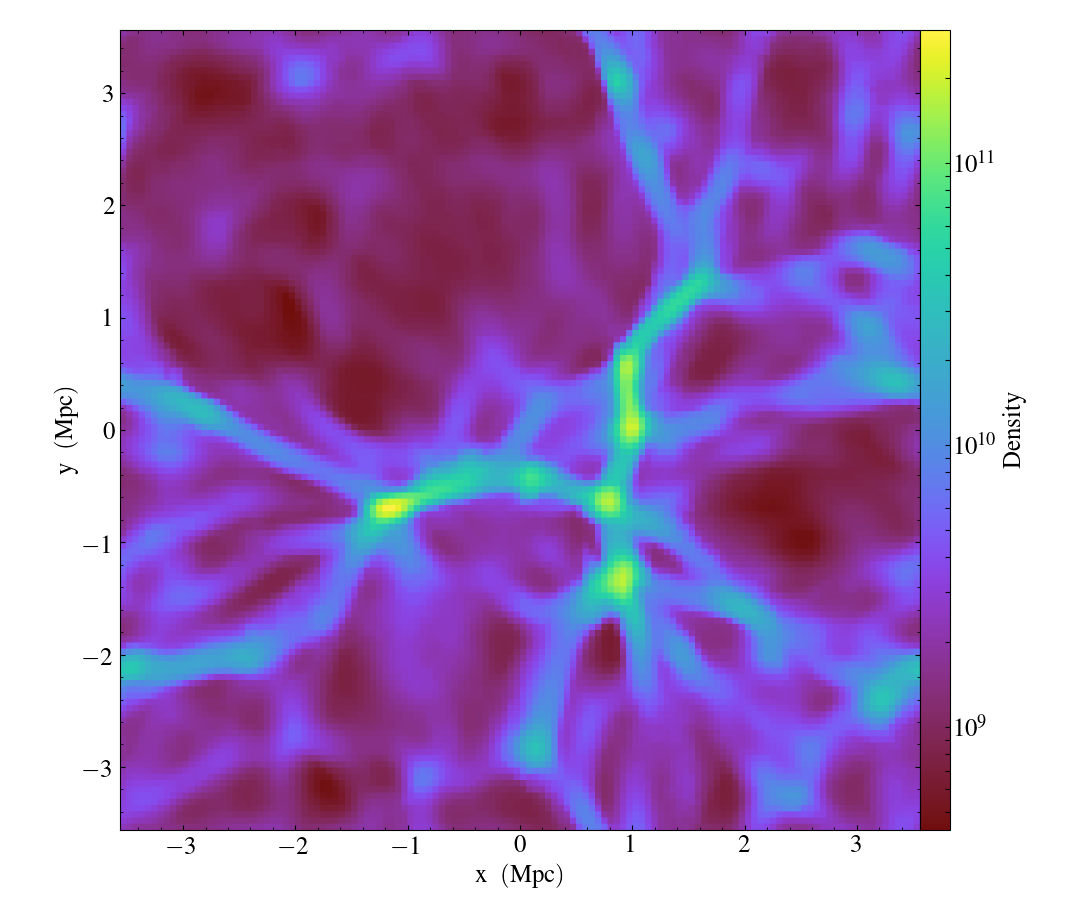
\includegraphics[scale=0.5]{./Visualization/yt_Nyx_density_slice.png}
  \caption{Slice plot of $128^3$ Nyx simulation using \yt.}
  \label{fig:yt_Nyx_slice_plot}
\end{figure}

\begin{lstlisting}[language=python,breaklines=true]
In [12]: sc = yt.create_scene(ds, field="density", lens_type="perspective")

In [13]: source = sc[0]

In [14]: source.tfh.set_bounds((1e8, 1e15))

In [15]: source.tfh.set_log(True)

In [16]: source.tfh.grey_opacity = True

In [17]: sc.show()
<Scene Object>:
Sources:
    source_00: <Volume Source>:YTRegion (plt00401): , center=[  1.09888770e+25   1.09888770e+25   1.09888770e+25] cm, left_edge=[ 0.  0.  0.] cm, right_edge=[  2.19777540e+25   2.19777540e+25   2.19777540e+25] cm transfer_function:None
Camera:
    <Camera Object>:
	position:[ 14.24501  14.24501  14.24501] code_length
	focus:[ 7.122505  7.122505  7.122505] code_length
	north_vector:[ 0.81649658 -0.40824829 -0.40824829]
	width:[ 21.367515  21.367515  21.367515] code_length
	light:None
	resolution:(512, 512)
Lens: <Lens Object>:
	lens_type:perspective
	viewpoint:[ 0.95423473  0.95423473  0.95423473] code_length

In [19]: sc.save()
yt : [INFO     ] 2017-05-23 10:15:07,825 Rendering scene (Can take a while).
yt : [INFO     ] 2017-05-23 10:15:07,825 Creating volume
yt : [INFO     ] 2017-05-23 10:15:07,996 Creating transfer function
yt : [INFO     ] 2017-05-23 10:15:07,997 Calculating data bounds. This may take a while.  Set the TranferFunctionHelper.bounds to avoid this.
yt : [INFO     ] 2017-05-23 10:15:16,471 Saving render plt00401_Render_density.png
\end{lstlisting}

The output of this is Figure~\ref{fig:yt_Nyx_vol_rend}.

\begin{figure}
  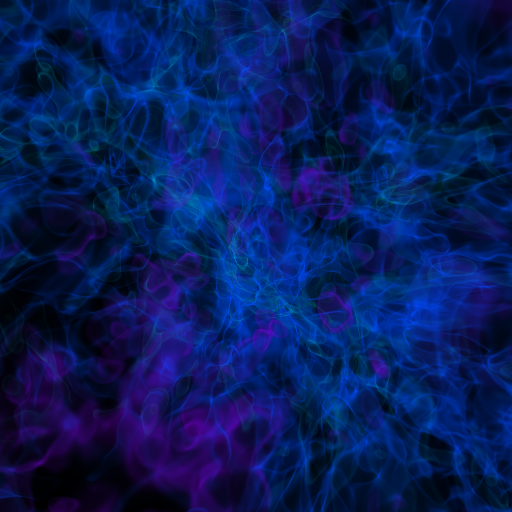
\includegraphics[scale=1.0]{./Visualization/yt_Nyx_density_vol_rend.png}
  \caption{Volume rendering of $128^3$ Nyx simulation using \yt. This
           corresponds to the same plot file used to generate the slice plot in
           Figure~\ref{fig:yt_Nyx_slice_plot}.}
  \label{fig:yt_Nyx_vol_rend}
\end{figure}

\subsection{Using \yt\ at NERSC (\emph{under development})}

Becase \yt\ is Python-based, it is portable and can be used in many software
environments. Here we focus on \yt's capabilities at NERSC, which provides
resources for performing both interactive and batch queue-based visualization
and analysis of \amrex\ data. Coupled with \yt's MPI and OpenMP parallelization
capabilities, this can enable high-throughput visualization and analysis
workflows.

\subsubsection{Interactive \yt\ with Jupyter notebooks}

Unlike \visit\ (\S\ref{sec:visit}), \yt\ has no client-server interface. Such
an interface is often crucial when one has large data sets generated on a
remote system, but wishes to visualize the data on a local workstation. Both
copying the data between the two systems, as well as visualizing the data
itself on a workstation, can be prohibitively slow.

Fortunately, NERSC has implemented several resources which allow one to
interact with \yt\ remotely, emulating a client-server model. In particular,
NERSC now hosts Jupyter notebooks which run IPython kernels on the Cori system;
this provides users access to the \texttt{\$HOME}, \texttt{/project}, and
\texttt{\$SCRATCH} file systems from a web browser-based Jupyter notebook.
\emph{\textbf{Please note that Jupyter hosting at NERSC is still under
development, and the environment may change without notice.}}

NERSC also provides Anaconda Python, which allows users to create their own
customizable Python environments. It is recommended to install \yt\ in such an
environment. One can do so with the following example:

\begin{lstlisting}
user@cori10:~> module load python/3.5-anaconda
user@cori10:~> conda create -p $HOME/yt-conda numpy
user@cori10:~> source activate $HOME/yt-conda
(/global/homes/u/user/yt-conda/) user@cori10:~> pip install yt
\end{lstlisting}

More information about Anaconda Python at NERSC is here:
\url{http://www.nersc.gov/users/data-analytics/data-analytics/python/anaconda-python/}.

One can then configure this Anaconda environment to run in a Jupyter notebook
hosted on the Cori system. Currently this is available in two places: on
\url{https://ipython.nersc.gov}, and on \url{https://jupyter-dev.nersc.gov}.
The latter likely reflects what the stable, production environment for Jupyter
notebooks will look like at NERSC, but it is still under development and
subject to change. To load this custom Python kernel in a Jupyter notebook,
follow the instructions at this URL under the ``Custom Kernels'' heading:
\url{http://www.nersc.gov/users/data-analytics/data-analytics/web-applications-for-data-analytics}.
After writing the appropriate \texttt{kernel.json} file, the custom kernel will
appear as an available Jupyter notebook. Then one can interactively visualize
\amrex\ plot files in the web browser.\footnote{It is convenient to use the
magic command \texttt{\%matplotlib inline} in order to render matplotlib
figures in the same browser window as the notebook, as opposed to displaying it
as a new window.}

\subsubsection{Parallel \yt}

Besides the benefit of no longer needing to move data back and forth between
NERSC and one's local workstation to do visualization and analysis, an
additional feature of \yt\ which takes advantage of the computational resources
at NERSC is its parallelization capabilities. \yt\ supports both MPI- and
OpenMP-based parallelization of various tasks, which are discussed here:
\url{http://yt-project.org/doc/analyzing/parallel_computation.html}.

Configuring \yt\ for MPI parallelization at NERSC is a more complex task than
discussed on the official \yt\ documentation; the command \texttt{pip install
mpi4py} is not sufficient. Rather, one must compile \texttt{mpi4py} from source
using the Cray compiler wrappers \texttt{cc}, \texttt{CC}, and \texttt{ftn} on
Cori. Instructions for compiling \texttt{mpi4py} at NERSC are provided here:
\url{http://www.nersc.gov/users/data-analytics/data-analytics/python/anaconda-python/#toc-anchor-3}.
After \texttt{mpi4py} has been compiled, one can use the regular Python
interpreter in the Anaconda environment as normal; when executing \yt\
operations which support MPI parallelization, the multiple MPI processes will
spawn automatically.

Although several components of \yt\ support MPI parallelization, a few are particularly useful:
\begin{itemize}
  \item \textbf{Time series analysis.} Often one runs a simulation for many
time steps and periodically writes plot files to disk for visualization and
post-processing. \yt\ supports parallelization over time series data via the
\texttt{DatasetSeries} object. \yt\ can iterate over a \texttt{DatasetSeries}
in parallel, with different MPI processes operating on different elements of
the series. This page provides more documentation:
\url{http://yt-project.org/doc/analyzing/time_series_analysis.html#time-series-analysis}.

  \item \textbf{Volume rendering}. \yt\ implements spatial decomposition among
MPI processes for volume rendering procedures, which can be computationally
expensive. Note that \yt\ also implements OpenMP parallelization in volume
rendering, and so one can execute volume rendering with a hybrid MPI+OpenMP
approach. See this URL for more details:
\url{http://yt-project.org/doc/visualizing/volume_rendering.html?highlight=openmp#openmp-parallelization}.

  \item \textbf{Generic parallelization over multiple objects.} Sometimes one
wishes to loop over a series which is not a \texttt{DatasetSeries}, e.g.,
performing translational or rotational operations on a camera to make a volume
rendering in which the field of view moves through the simulation. In this
case, one is applying a set of operations on a single object (a single plot
file), rather than over a time series of data. For this workflow, \yt\ provides
the \texttt{parallel\_objects()} function. See this URL for more details:
\url{http://yt-project.org/doc/analyzing/parallel_computation.html#parallelizing-over-multiple-objects}.

An example of MPI parallelization in \yt\ is shown below, where one animates a
time series of plot files from an IAMR simulation while revolving the camera
such that it completes two full revolutions over the span of the animation:

\begin{lstlisting}[language=python,breaklines=true]
import yt
import glob
import numpy as np

yt.enable_parallelism()

base_dir1 = '/global/cscratch1/sd/user/Nyx_run_p1'
base_dir2 = '/global/cscratch1/sd/user/Nyx_run_p2'
base_dir3 = '/global/cscratch1/sd/user/Nyx_run_p3'

glob1 = glob.glob(base_dir1 + '/plt*')
glob2 = glob.glob(base_dir2 + '/plt*')
glob3 = glob.glob(base_dir3 + '/plt*')

files = sorted(glob1 + glob2 + glob3)

ts = yt.DatasetSeries(files, parallel=True)

frame = 0
num_frames = len(ts)
num_revol = 2

slices = np.arange(len(ts))

for i in yt.parallel_objects(slices):
    sc = yt.create_scene(ts[i], lens_type='perspective', field='z_velocity')

    source = sc[0]
    source.tfh.set_bounds((1e-2, 9e+0))
    source.tfh.set_log(False)
    source.tfh.grey_opacity = False

    cam = sc.camera

    cam.rotate(num_revol*(2.0*np.pi)*(i/num_frames),
               rot_center=np.array([0.0, 0.0, 0.0]))

    sc.save(sigma_clip=5.0)
\end{lstlisting}

When executed on 4 CPUs on a Haswell node of Cori, the output looks like the following:

\begin{lstlisting}[breaklines=true]
user@nid00009:~/yt_vis/> srun -n 4 -c 2 --cpu_bind=cores python make_yt_movie.py
yt : [INFO     ] 2017-05-23 16:51:33,565 Global parallel computation enabled: 0 / 4
yt : [INFO     ] 2017-05-23 16:51:33,565 Global parallel computation enabled: 2 / 4
yt : [INFO     ] 2017-05-23 16:51:33,566 Global parallel computation enabled: 1 / 4
yt : [INFO     ] 2017-05-23 16:51:33,566 Global parallel computation enabled: 3 / 4
P003 yt : [INFO     ] 2017-05-23 16:51:33,957 Parameters: current_time              = 0.103169376949795
P003 yt : [INFO     ] 2017-05-23 16:51:33,957 Parameters: domain_dimensions         = [128 128 128]
P003 yt : [INFO     ] 2017-05-23 16:51:33,957 Parameters: domain_left_edge          = [ 0.  0.  0.]
P003 yt : [INFO     ] 2017-05-23 16:51:33,958 Parameters: domain_right_edge         = [ 6.28318531  6.28318531  6.28318531]
P000 yt : [INFO     ] 2017-05-23 16:51:33,969 Parameters: current_time              = 0.0
P000 yt : [INFO     ] 2017-05-23 16:51:33,969 Parameters: domain_dimensions         = [128 128 128]
P002 yt : [INFO     ] 2017-05-23 16:51:33,969 Parameters: current_time              = 0.0687808060674485
P000 yt : [INFO     ] 2017-05-23 16:51:33,969 Parameters: domain_left_edge          = [ 0.  0.  0.]
P002 yt : [INFO     ] 2017-05-23 16:51:33,969 Parameters: domain_dimensions         = [128 128 128]
P000 yt : [INFO     ] 2017-05-23 16:51:33,970 Parameters: domain_right_edge         = [ 6.28318531  6.28318531  6.28318531]
P002 yt : [INFO     ] 2017-05-23 16:51:33,970 Parameters: domain_left_edge          = [ 0.  0.  0.]
P002 yt : [INFO     ] 2017-05-23 16:51:33,970 Parameters: domain_right_edge         = [ 6.28318531  6.28318531  6.28318531]
P001 yt : [INFO     ] 2017-05-23 16:51:33,973 Parameters: current_time              = 0.0343922351851018
P001 yt : [INFO     ] 2017-05-23 16:51:33,973 Parameters: domain_dimensions         = [128 128 128]
P001 yt : [INFO     ] 2017-05-23 16:51:33,974 Parameters: domain_left_edge          = [ 0.  0.  0.]
P001 yt : [INFO     ] 2017-05-23 16:51:33,974 Parameters: domain_right_edge         = [ 6.28318531  6.28318531  6.28318531]
P000 yt : [INFO     ] 2017-05-23 16:51:34,589 Rendering scene (Can take a while).
P000 yt : [INFO     ] 2017-05-23 16:51:34,590 Creating volume
P003 yt : [INFO     ] 2017-05-23 16:51:34,592 Rendering scene (Can take a while).
P002 yt : [INFO     ] 2017-05-23 16:51:34,592 Rendering scene (Can take a while).
P003 yt : [INFO     ] 2017-05-23 16:51:34,593 Creating volume
P002 yt : [INFO     ] 2017-05-23 16:51:34,593 Creating volume
P001 yt : [INFO     ] 2017-05-23 16:51:34,606 Rendering scene (Can take a while).
P001 yt : [INFO     ] 2017-05-23 16:51:34,607 Creating volume
\end{lstlisting}

Because the \texttt{parallel\_objects()} function transforms the loop into a
data-parallel problem, this procedure strong scales nearly perfectly to an
arbitrarily large number of MPI processes, allowing for rapid rendering of
large time series of data.

\end{itemize}


\chapter{Profiling}\label{Chap:Profiling}
\amrex-based application codes can be instrumented using AMReX-specific performance
profiling tools that take into account the hierarchical nature of the mesh in 
most AMReX-based applications.  These codes can be instrumented for varying levels of 
profiling detail.  The broad-brush C++ instrumentation is as follows:

\section{Instrumenting the Code} 
\subsection{C++} 

\begin{lstlisting}[language=cpp]
void YourClass::YourFunction() 
{
  BL_PROFILE("YourClass::YourFunction()");  // this name can be any string

  // your function code
}
\end{lstlisting}

For other timers within an already instrumented function, add:
 
\begin{lstlisting}[language=cpp]
      BL_PROFILE_VAR("Flaten::FORT_FLATENX()", anyname);  // add this before
        FORT_FLATENX(arg1, arg2);
      BL_PROFILE_VAR_STOP(anyname);   // add this after, using the same name
\end{lstlisting}
 
if you want to use the same name within the same scope, you can use:
 
\begin{lstlisting}[language=cpp]
      BL_PROFILE_VAR("MyFuncs()", myfuncs);  // the first one
        MyFunc_0(arg);
      BL_PROFILE_VAR_STOP(myfuncs);
      ...
      BL_PROFILE_VAR_START(myfuncs);
        MyFunc_1(arg);
      BL_PROFILE_VAR_STOP(myfuncs);
\end{lstlisting}
 
or create a profiling variable without starting, then start/stop:
 
\begin{lstlisting}[language=cpp]
      BL_PROFILE_VAR_NS("MyFuncs()", myfuncs);  // dont start the timer
      ...
      BL_PROFILE_VAR_START(myfuncs);
        MyFunc_0(arg);
      BL_PROFILE_VAR_STOP(myfuncs);
      ...
      BL_PROFILE_VAR_START(myfuncs);
        MyFunc_1(arg);
      BL_PROFILE_VAR_STOP(myfuncs);
\end{lstlisting}

\subsection{Fortran90} 

Fortran90 functions can also be instrumented with the following calls:
 
\begin{lstlisting}[language=fortran]
call bl_proffortfuncstart("my_function")
...
call bl_proffortfuncstop("my_function")
\end{lstlisting}
 
Note that the start and stop calls must be matched and the profiling output will warn of any 
{\tt bl\_proffortfuncstart} calls that were not stopped with {\tt bl\_proffortfuncstop} calls
(in debug mode only).  You will need to add {\tt bl\_proffortfuncstop}
before any returns and at the end of the function or at the point in the
function you want to stop profiling. 

\section{Types of Profiling} 

Currently you have two options for AMReX-specific profiling.  If you set {\tt TINY\_PROFILE = TRUE}
in your GNUMakefile then at the end of the run, a summary of exclusive and inclusive function times 
will be written to stdout.

If you set {\tt PROFILE = TRUE} then a {\tt bl\_prof} directory will be written that contains 
detailed per-task timings of the code.    An exclusive-only set of function timings will be written to stdout

If, in addition to  {\tt PROFILE = TRUE}, you set {\tt TRACE\_PROFILE = TRUE}, then the profiler keeps track
of when each profiled function is called and  the {\tt bl\_prof} directory will include the function call stack.   
This is especially useful when core functions, such as {\tt FillBoundary} can be called from many different regions of the code.
Part of the trace profiling is the ability to set regions in the code which can be analyzed for profiling information independently from other regions. 

If, in addition to  {\tt PROFILE = TRUE}, you set {\tt COMM\_PROFILE = TRUE}, then the {\tt bl\_prof} directory 
will contain additional information about MPI communication (point-to-point timings, data volume, barrier/reduction times, etc.).  {\tt TRACE\_PROFILE = TRUE} and {\tt COMM\_PROFILE = TRUE} can be set together.

The AMReX-specific profiling tools are currently under development and this documentation will reflect the latest 
status in the development branch.

\section{Sample Output}

Sample output from {\tt TINY\_PROFILE = TRUE} can look like the following:


\begin{lstlisting}[basicstyle=\tiny,tabsize=1]

TinyProfiler total time across processes [min...avg...max]: 1.765...1.765...1.765
---------------------------------------------------------------------------------
Name                          NCalls   Excl. Min   Excl. Avg   Excl. Max   Max  %
---------------------------------------------------------------------------------
mfix_level::EvolveFluid       1        1.602       1.668       1.691       95.83%
FabArray::FillBoundary()      11081    0.02195     0.03336     0.06617      3.75%
FabArrayBase::getFB()         22162    0.02031     0.02147     0.02275      1.29%
PC<...>::WriteAsciiFile()     1        0.00292     0.004072    0.004551     0.26%


---------------------------------------------------------------------------------
Name                          NCalls   Incl. Min   Incl. Avg  Incl. Max    Max  %
---------------------------------------------------------------------------------
mfix_level::Evolve()          1        1.69        1.723      1.734        98.23%
mfix_level::EvolveFluid       1        1.69        1.723      1.734        98.23%
FabArray::FillBoundary()      11081    0.04236     0.05485    0.08826       5.00%
FabArrayBase::getFB()         22162    0.02031     0.02149    0.02275       1.29%

\end{lstlisting}

\section{\tt AMRProfParser} 

{\tt AMRProfParser} is a tool for processing and analyzing the {\tt bl\_prof} database.  It is a
command line application that can create performance summaries, plotfiles showing
point to point communication and timelines, HTML call trees, communication call
statistics, function timing graphs, and other data products.  The parser's data
services functionality can be called from an interactive environment such as {\tt Amrvis},
from a sidecar for dynamic performance optimization, and from other utilities such as
the command line version of the parser itself.  It has been integrated into {\tt Amrvis}
for visual interpretation of the data allowing {\tt Amrvis} to open the {\tt bl\_prof} database
like a plotfile but with interfaces appropriate to profiling data. AMRProfParser
and {\tt Amrvis} can be run in parallel both interactively and in batch mode.

\section{CrayPat}

The profiling suite available on Cray XC systems is Cray Performance
Measurement and Analysis Tools
(``CrayPat'')\footnote{\url{https://pubs.cray.com/content/S-2376/6.4.6/cray-performance-measurement-and-analysis-tools-user-guide-646-s-2376}}.
Most CrayPat functionality is supported for all compilers available in the Cray
``programming environments`` (modules which begin ``\texttt{PrgEnv-}'');
however, a few features, chiefly the ``Reveal'' tool, are supported only on
applications compiled with Cray's compiler
CCE\footnote{\url{https://pubs.cray.com/content/S-2179/8.5/cray-c-and-c++-reference-manual-85}}\footnote{\url{https://pubs.cray.com/content/S-3901/8.5/cray-fortran-reference-manual-85}}.

CrayPat supports both high-level profiling tools, as well as fine-grained
performance analysis, such as reading hardware counters. The default behavior
uses sampling to identify the most time-consuming functions in an application.

\subsection{High-level application profiling}

The simplest way to obtain a high-level overview of an application's performance consists of the following steps:

\begin{enumerate}
    \item Load the \texttt{perftools-base} module, then the
        \texttt{perftools-lite} module. (The modules will not work if loaded in
        the opposite order.)
    \item Compile the application with the Cray compiler wrappers \texttt{cc},
        \texttt{CC}, and/or \texttt{ftn}. This works with any of the compilers
        available in the \texttt{PrgEnv-} modules. E.g., on the Cori system at
        NERSC, one can use the Intel, GCC, or CCE compilers. No extra compiler
        flags are necessary in order for CrayPat to work. CrayPat instruments
        the application, so the \texttt{perftools-} modules must be loaded
        before one compiles the application.
    \item Run the application as normal. No special flags are required. Upon
        application completion, CrayPat will write a few files to the directory
        from which the application was launched. The profiling database is a
        single file with the \texttt{.ap2} suffix.
    \item One can query the database in many different ways using the
        \texttt{pat\_report} command on the \texttt{.ap2} file. \texttt{pat\_report} is
        available on login nodes, so the analysis need not be done on a compute node.
        Querying the database with no arguments to \texttt{pat\_report} prints several
        different profiling reports to STDOUT, including a list of the most
        time-consuming regions in the application. The output of this command can be
        long, so it can be convenient to pipe the output to a pager or a file. A
        portion of the output from \texttt{pat\_report <file>.ap2} is shown below:

\begin{verbatim}
Table 1:  Profile by Function

  Samp% |    Samp |  Imb. |  Imb. | Group
        |         |  Samp | Samp% |  Function
        |         |       |       |   PE=HIDE

 100.0% | 5,235.5 |    -- |    -- | Total
|-----------------------------------------------------------------------------
|  50.2% | 2,628.5 |    -- |    -- | USER
||----------------------------------------------------------------------------
||   7.3% |   383.0 |  15.0 |  5.0% | eos_module_mp_iterate_ne_
||   5.7% |   300.8 | 138.2 | 42.0% | amrex_deposit_cic
||   5.1% |   265.2 |  79.8 | 30.8% | update_dm_particles
||   2.8% |   147.2 |   5.8 |  5.0% | fort_fab_setval
||   2.6% |   137.2 |  48.8 | 34.9% | amrex::ParticleContainer<>::Where
||   2.6% |   137.0 |  11.0 |  9.9% | ppm_module_mp_ppm_type1_
||   2.5% |   133.0 |  24.0 | 20.4% | eos_module_mp_nyx_eos_t_given_re_
||   2.1% |   107.8 |  33.2 | 31.4% | amrex::ParticleContainer<>::IncrementWithTotal
||   1.7% |    89.2 |  19.8 | 24.2% | f_rhs_
||   1.4% |    74.0 |   7.0 | 11.5% | riemannus_
||   1.1% |    56.0 |   2.0 |  4.6% | amrex::VisMF::Write
||   1.0% |    50.5 |   1.5 |  3.8% | amrex::VisMF::Header::CalculateMinMax
||============================================================================
|  28.1% | 1,471.0 |    -- |    -- | ETC
||----------------------------------------------------------------------------
||   7.4% |   388.8 |  10.2 |  3.4% | __intel_mic_avx512f_memcpy
||   6.9% |   362.5 |  45.5 | 14.9% | CVode
||   3.1% |   164.5 |   8.5 |  6.6% | __libm_log10_l9
||   2.9% |   149.8 |  29.2 | 21.8% | _INTERNAL_25_______src_kmp_barrier_cpp_5de9139b::__kmp_hyper_barrier_gather
||============================================================================
|  16.8% |   879.8 |    -- |    -- | MPI
||----------------------------------------------------------------------------
||   5.1% |   266.0 | 123.0 | 42.2% | MPI_Allreduce
||   4.2% |   218.2 | 104.8 | 43.2% | MPI_Waitall
||   2.9% |   151.8 |  78.2 | 45.4% | MPI_Bcast
||   2.6% |   135.0 |  98.0 | 56.1% | MPI_Barrier
||   2.0% |   105.8 |   5.2 |  6.3% | MPI_Recv
||============================================================================
|   1.9% |    98.2 |    -- |    -- | IO
||----------------------------------------------------------------------------
||   1.8% |    93.8 |   6.2 |  8.3% | read
||============================================================================
\end{verbatim}


\end{enumerate}

\section{IPM - Cross-Platform Integrated Performance Monitoring}

IPM provides portable profiling capabilities across HPC platforms,
including support on selected Cray and IBM machines (cori and (TODO:
verify it works on) summit).  Running an IPM instrumented binary generates
a summary of number of calls and time spent on MPI communication library
functions.  In addition, hardware performance counters can also be
collected through PAPI.

Detailed instructions can be found at \footnote{\url{http://ipm-hpc.sourceforge.net/userguide.html}} and
\footnote{\url{https://www.nersc.gov/users/software/performance-and-debugging-tools/ipm/}}.

\subsection{Building with IPM on cori}

Steps:
\begin{enumerate}
\item Run {\tt module load ipm}.
\item Build code as normal with {\tt make}.
\item Re-run the link command (e.g. cut-and-paste) with {\tt \$IPM} added to the end of the line.
\end{enumerate}

\subsection{Running with IPM on cori}

\begin{enumerate}
\item Set environment variables: {\tt export IPM\_REPORT=full IPM\_LOG=full IPM\_LOGDIR=$<$dir$>$}
\item Results will be printed to stdout and an xml file generated in the directory specified by {\tt IPM\_LOGDIR}.
\item Post-process the xml with {\tt ipm\_parse -html $<$xmlfile$>$}, which produces an directory with html.
\end{enumerate}

\subsection{Summary MPI Profile}

Example MPI profile output:

\begin{verbatim}
##IPMv2.0.5########################################################
#
# command   : /global/cscratch1/sd/cchan2/projects/lbl/BoxLib/Tests/LinearSolvers/C_CellMG/./main3d.intel.MPI.OMP.ex.ipm inputs.3d.25600 
# start     : Tue Aug 15 17:34:23 2017   host      : nid11311        
# stop      : Tue Aug 15 17:34:35 2017   wallclock : 11.54
# mpi_tasks : 128 on 32 nodes            %comm     : 32.51
# mem [GB]  : 126.47                     gflop/sec : 0.00
#
#           :       [total]        <avg>          min          max
# wallclock :       1188.42         9.28         8.73        11.54 
# MPI       :        386.31         3.02         2.51         4.78 
# %wall     :
#   MPI     :                      32.52        24.36        41.44 
# #calls    :
#   MPI     :       5031172        39306        23067        57189
# mem [GB]  :        126.47         0.99         0.98         1.00 
#
#                             [time]        [count]        <%wall>
# MPI_Allreduce               225.72         567552          18.99
# MPI_Waitall                  92.84         397056           7.81
# MPI_Recv                     29.36            193           2.47
# MPI_Isend                    25.04        2031810           2.11
# MPI_Irecv                     4.35        2031810           0.37
# MPI_Allgather                 2.60            128           0.22
# MPI_Barrier                   2.24            512           0.19
# MPI_Gatherv                   1.70            128           0.14
# MPI_Comm_dup                  1.23            256           0.10
# MPI_Bcast                     1.14            256           0.10
# MPI_Send                      0.06            319           0.01
# MPI_Reduce                    0.02            128           0.00
# MPI_Comm_free                 0.01            128           0.00
# MPI_Comm_group                0.00            128           0.00
# MPI_Comm_size                 0.00            256           0.00
# MPI_Comm_rank                 0.00            256           0.00
# MPI_Init                      0.00            128           0.00
# MPI_Finalize                  0.00            128           0.00
\end{verbatim}

The total, average, minimum, and maximum wallclock and MPI times across ranks is shown.
The memory footprint is also collected.
Finally, results include number of calls and total time spent in each type of MPI call.

\subsection{PAPI Performance Counters}

To collect performance counters, set {\tt IPM\_HPM=$<$list$>$}, where the list is a comma-separated
list of PAPI counters.  For example: {\tt export IPM\_HPM=PAPI\_L2\_TCA,PAPI\_L2\_TCM}.

For reference, here is the list of available counters on cori, which can be found by running {\tt papi\_avail}:
\begin{verbatim}
    Name        Code    Avail Deriv Description (Note)
PAPI_L1_DCM  0x80000000  Yes   No   Level 1 data cache misses
PAPI_L1_ICM  0x80000001  Yes   No   Level 1 instruction cache misses
PAPI_L1_TCM  0x80000006  Yes   Yes  Level 1 cache misses
PAPI_L2_TCM  0x80000007  Yes   No   Level 2 cache misses
PAPI_TLB_DM  0x80000014  Yes   No   Data translation lookaside buffer misses
PAPI_L1_LDM  0x80000017  Yes   No   Level 1 load misses
PAPI_L2_LDM  0x80000019  Yes   No   Level 2 load misses
PAPI_STL_ICY 0x80000025  Yes   No   Cycles with no instruction issue
PAPI_BR_UCN  0x8000002a  Yes   Yes  Unconditional branch instructions
PAPI_BR_CN   0x8000002b  Yes   No   Conditional branch instructions
PAPI_BR_TKN  0x8000002c  Yes   No   Conditional branch instructions taken
PAPI_BR_NTK  0x8000002d  Yes   Yes  Conditional branch instructions not taken
PAPI_BR_MSP  0x8000002e  Yes   No   Conditional branch instructions mispredicted
PAPI_TOT_INS 0x80000032  Yes   No   Instructions completed
PAPI_LD_INS  0x80000035  Yes   No   Load instructions
PAPI_SR_INS  0x80000036  Yes   No   Store instructions
PAPI_BR_INS  0x80000037  Yes   No   Branch instructions
PAPI_RES_STL 0x80000039  Yes   No   Cycles stalled on any resource
PAPI_TOT_CYC 0x8000003b  Yes   No   Total cycles
PAPI_LST_INS 0x8000003c  Yes   Yes  Load/store instructions completed
PAPI_L1_DCA  0x80000040  Yes   Yes  Level 1 data cache accesses
PAPI_L1_ICH  0x80000049  Yes   No   Level 1 instruction cache hits
PAPI_L1_ICA  0x8000004c  Yes   No   Level 1 instruction cache accesses
PAPI_L2_TCH  0x80000056  Yes   Yes  Level 2 total cache hits
PAPI_L2_TCA  0x80000059  Yes   No   Level 2 total cache accesses
PAPI_REF_CYC 0x8000006b  Yes   No   Reference clock cycles
\end{verbatim}

Due to hardware limitations, there is a limit to which counters can be
collected simultaneously in a single run.  Some counters may map to the
same registers and thus cannot be collected at the same time.

\subsection{Example HTML Performance Summary}

Running {\tt ipm\_parse -html $<$xmlfile$>$} on the generated xml file
will produce an HTML document that includes summary performance numbers
and automatically generated figures.  Some examples are shown here.

\begin{figure}
  \begin{center}
    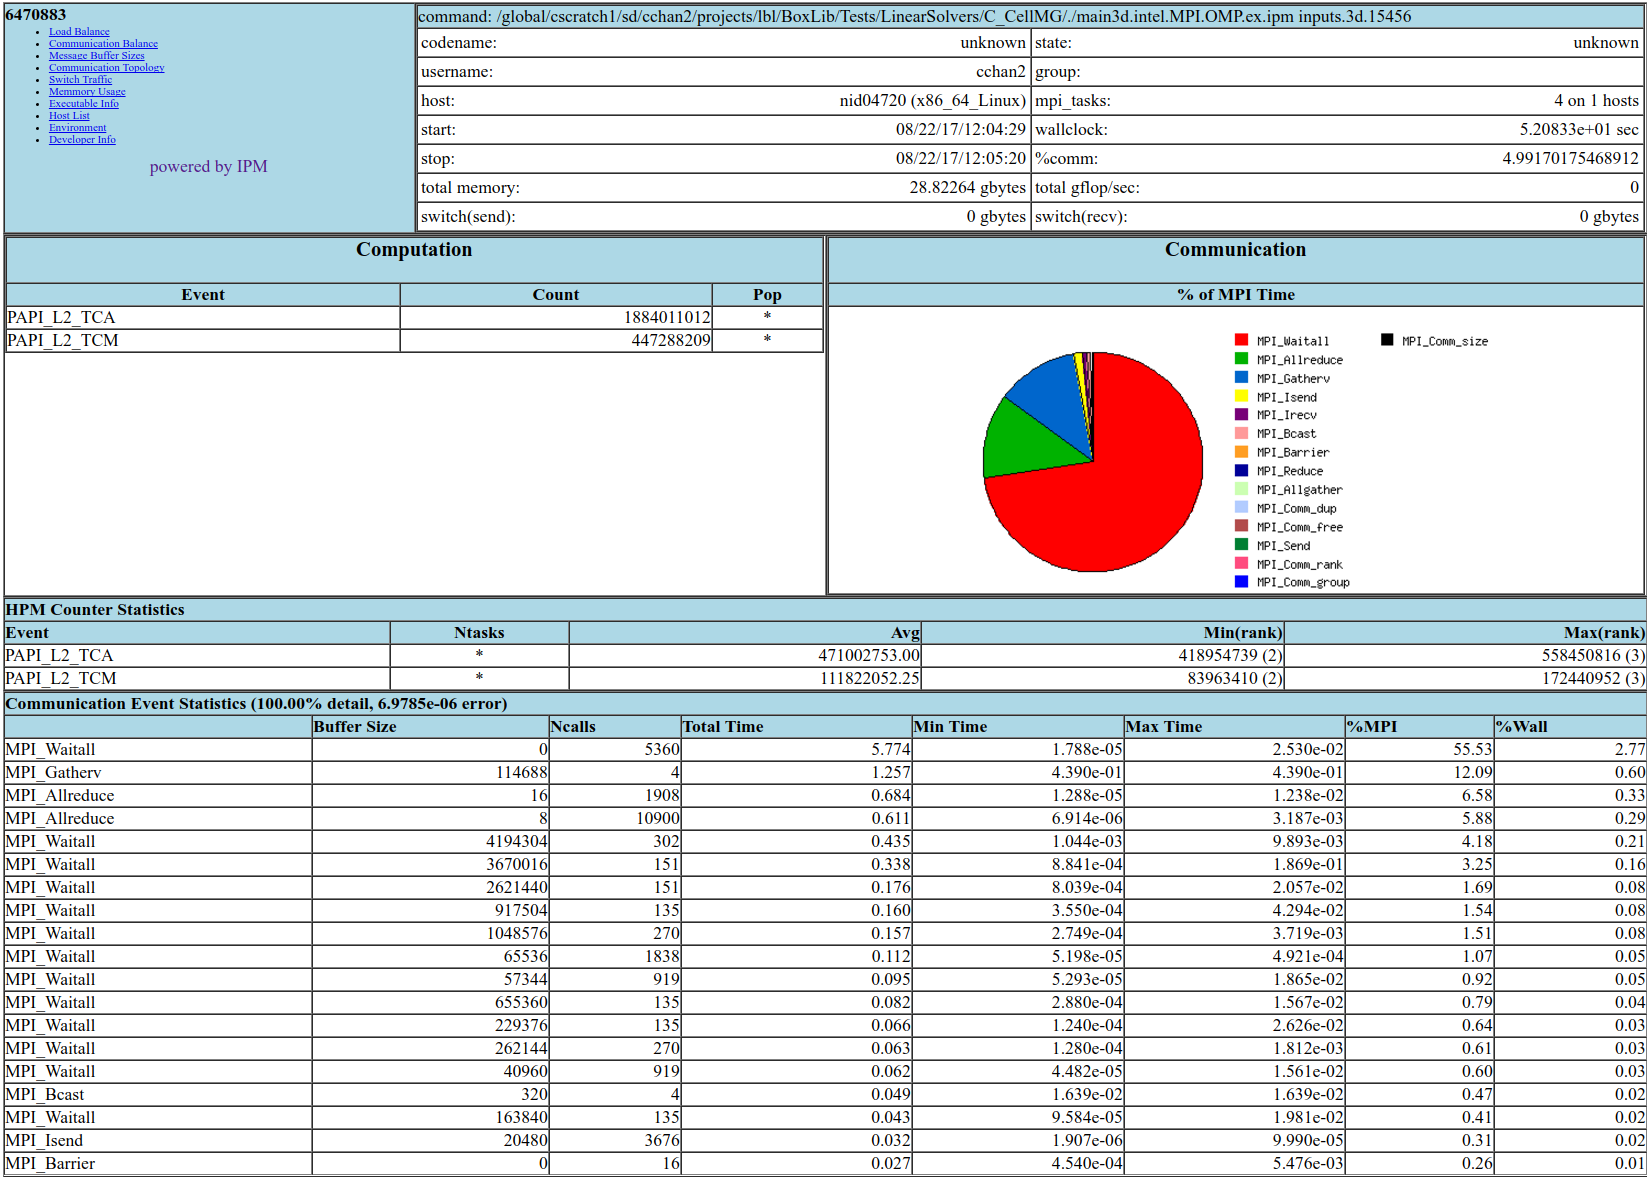
\includegraphics[width=\columnwidth]{Profiling/figs/summary.png}
  \end{center}
  \caption{
    Sample performance summary generated by IPM
  }
  \label{fig:ipm-summary}
\end{figure}

\begin{figure}
  \begin{center}
    \subfloat[Timings]{
      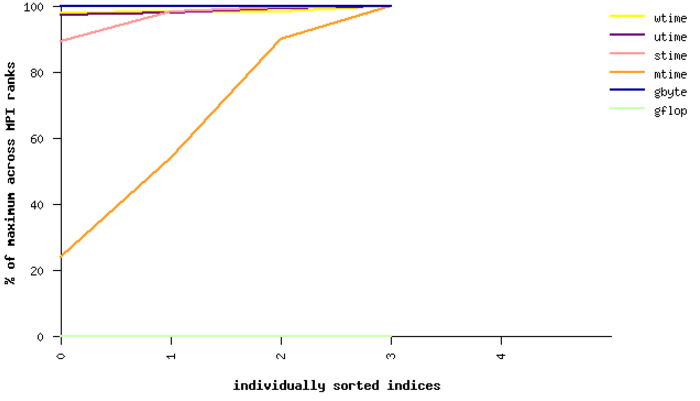
\includegraphics[width=0.49\columnwidth]{Profiling/figs/timings.png}
    }
    \subfloat[PAPI Counters]{
      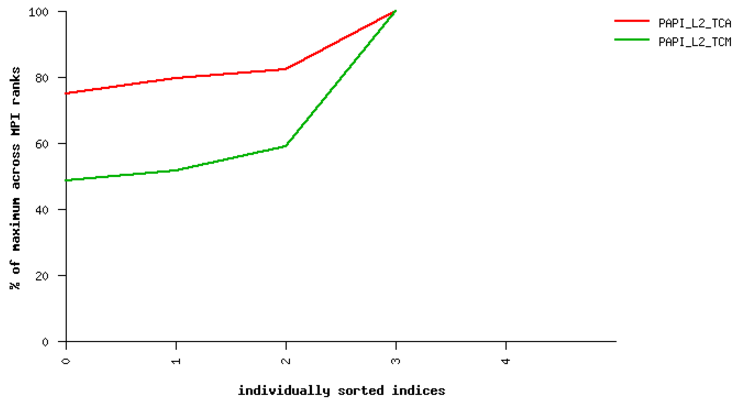
\includegraphics[width=0.49\columnwidth]{Profiling/figs/papi.png}
    } \\
    \subfloat[MPI Time by Function]{
      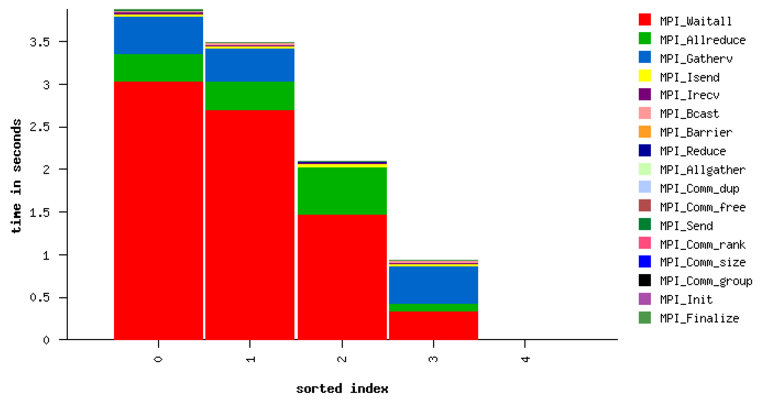
\includegraphics[width=0.49\columnwidth]{Profiling/figs/mpi.png}
    }
    \subfloat[MPI Time by Message Size]{
      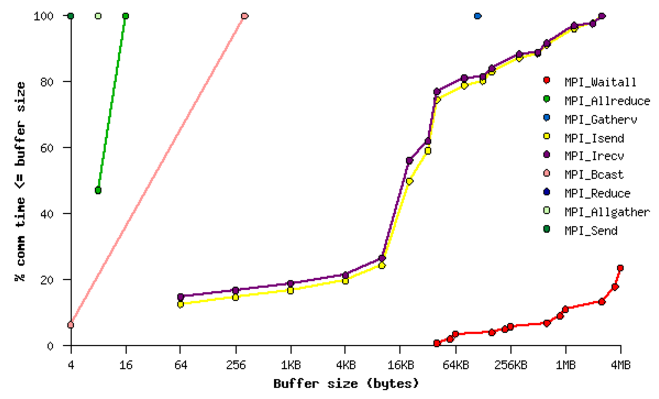
\includegraphics[width=0.49\columnwidth]{Profiling/figs/msgsizes.png}
    } \\
    \subfloat[Point-to-Point Communication Volume]{
      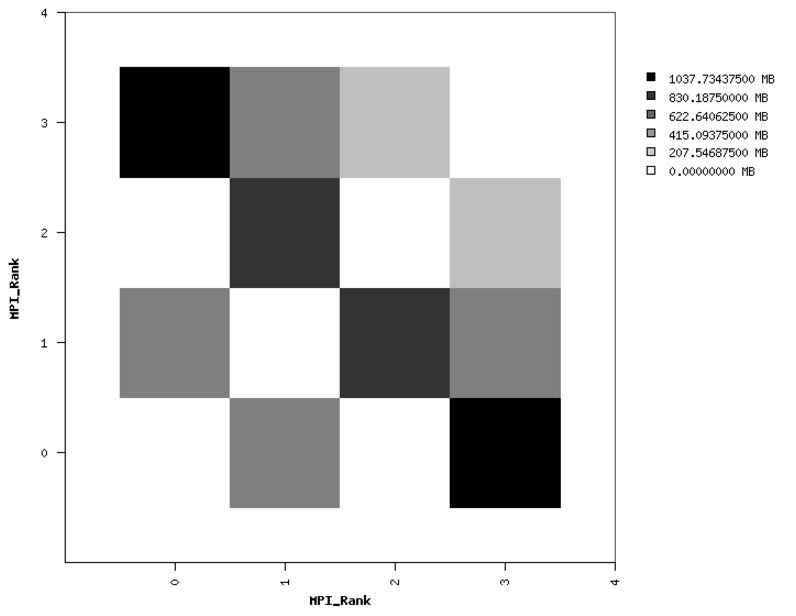
\includegraphics[width=0.49\columnwidth]{Profiling/figs/commtopo.png}
    }
  \end{center}
  \caption{
    Sample performance graphs generated by IPM
  }
  \label{fig:ipm-graphs}
\end{figure}


%\chapter{Debugging}\label{Chap:Debugging}
%On debugging


\chapter{CVODE}\label{Chap:CVODE}
\amrex\ supports ODE integration using the \cvode\ solver,\footnote{\url{https://computation.llnl.gov/projects/sundials/cvode}} which is part of the \sundials\ framework.\footnote{\url{https://computation.llnl.gov/projects/sundials}}
\cvode\ contains solvers for stiff and non-stiff ODEs, and as such is well suited for solving e.g., the complex chemistry networks in combustion simulations, or the nuclear reaction networks in astrophysical simulations.

Most of \cvode\ is written in C, but many functions also come with two distinct Fortran interfaces.
One interface is \fcvode, which is bundled with the stable release of \cvode.
Its usage is described in the CVODE documentation (\url{https://computation.llnl.gov/sites/default/files/public/cv_guide.pdf}).

The second, newer Fortran interface to \cvode\ uses the \texttt{iso\_c\_binding} feature of the Fortran 2003 standard to implement a ``thinner,'' more direct interface to the C functions in \cvode.
In contrast to the \fcvode\ interface, the Fortran 2003 interface calls C functions directly, with identical arguments.
When compiling \cvode, one need not build the Fortran interface to \cvode\ at all to use this new interface.
The examples provided in \amrex\ use this new interface.

To use \cvode\ in an \amrex\ application, follow these steps:

\begin{enumerate}

  \item Obtain the \cvode\ source code, which is hosted here: \url{https://computation.llnl.gov/projects/sundials/sundials-software}.

  One can download either the complete \sundials\ package, or just the \cvode\ components.

  \item Unpack the \cvode/\sundials\ tarball, and create a new ``build'' directory (it can be anywhere).

  \item Navigate to the new, empty build directory, and type

  \begin{verbatim}
  cmake \
    -DCMAKE_INSTALL_PREFIX:PATH=/path/to/install/dir \
    /path/to/cvode/or/sundials/top/level/source/dir
  \end{verbatim}

  The \texttt{CMAKE\_INSTALL\_DIR} option tells CMake where to install the libraries.
  Note that CMake will attempt to deduce the compilers automatically, but respects certain environment variables if they are defined, such as \texttt{CC} (for the C compiler), \texttt{CXX} (for the C++ compiler), and \texttt{FC} (for the Fortran compiler).
  So one may modify the above CMake invocation to be something like the following:

  \begin{verbatim}
  CC=/path/to/gcc \
  CXX=/path/to/g++ \
  FC=/path/to/gfortran \
    cmake \
    -DCMAKE_INSTALL_PREFIX:PATH=/path/to/install/dir \
    /path/to/cvode/or/sundials/top/level/source/dir
  \end{verbatim}

  \item In the \texttt{GNUmakefile} for the \amrex\ application which uses the Fortran 2003 interface to \cvode, add \texttt{USE\_CVODE = TRUE}, which will compile the Fortran 2003 interfaces and link the \cvode\ libraries.
  Note that one must define the \texttt{CVODE\_LIB\_DIR} environment variable to point to the location where the libraries are installed.
\end{enumerate}


%------------------------------------------------------------------------------
\backmatter

% \renewcommand\bibname{References}
% \addcontentsline{toc}{chapter}{References}
% \bibliographystyle{plain}
% \bibliography{refs,Verification/verification,Gravity/gr}

%\cleardoublepage
%\phantomsection
%\addcontentsline{toc}{chapter}{Index}
%\printindex

\end{document}
